% \usepackage{nopageno}
% \usepackage{etex}

% \newcommand{ \red} [ 1]{{\color{red}#1}}
% \newcommand{ \blue} [ 1]{{\color{blue}#1}}
% \newcommand{ \cyan} [ 1]{{\color{cyan}#1}}
% \newcommand{ \magen} [ 1]{{\color{magenta}#1}}
% \newcommand{ \orange} [ 1]{{\color{orange}#1}}
% \newcommand{ \bfred }{\bf \color{red}}
% \newcommand{ \bfblue }{\bf \color{blue}}
% \newcommand{ \bfcyan} {\bf \color{cyan}}

\newcommand{\sref}[1]{Section~\ref{#1}}
\newcommand{\tref}[1]{Table~\ref{#1}}

% \newtheorem{definition}{Definition}[]
% \newtheorem{proposition}[definition]{Proposition}
% \newtheorem{fact}[definition]{Fact}
% \newtheorem{example}[definition]{Example}
% \newtheorem{theorem}{Theorem}
% \newtheorem{lemma}[definition]{Lemma}
% \newtheorem{condition}[definition]{Condition}
% \newtheorem{corollary}[definition]{Corollary}
% \newtheorem{remark}[definition]{Remark}
\newcommand{\ceil}[1]{\lceil{#1}\rceil}

% \usepackage[normalem]{ulem} \newcommand{\off}[1]{\st{#1}}
% \usepackage{booktabs}

% \newfont{\mycrnotice}{ptmr8t at 7pt}
% \newfont{\myconfname}{ptmri8t at 7pt}
% \let\crnotice\mycrnotice \let\confname\myconfname 
% \let\svthefootnote\thefootnote
% \newcommand\freefootnote[1]{\let\thefootnote\relax \footnotetext{#1}\let\thefootnote\svthefootnote }


\section{Risk-averse learning for latency minimization in mmWave integrated access and backhaul networks}
\label{sec:iab-safehaul}

% Methodologically, the majority of the existing works~\cite{pan2017joint, alizadeh2019load, huang2015joint, nguyen2020nonsmooth, rasekh2015interference, kwon2019joint, pizzo2017optimal, kulkarni2018max,9839601} focus on classic optimization techniques to solve the above-mentioned problem. However, given the large number of parameters involved, such formulations often result in non-convex problems that are too complex for real-time operations, but are nonetheless valuable indicators as performance upper bounds. Recently, some works focus on more practical solutions which can be deployed in real networks\cite{lei2020deep, ZHANG2021108248, 9473755}. Specifically, these works leverage \gls{rl} to tackle both resource allocation and/or path selection in IAB mmWave networks and demonstrate that \gls{rl}-based solutions achieve real-time performance. 

Regardless of the methodology,  prior works mostly aim at maximizing the network capacity~\cite{pan2017joint, alizadeh2019load, huang2015joint, nguyen2020nonsmooth, rasekh2015interference, kwon2019joint, pizzo2017optimal, kulkarni2018max}, minimizing latency~\cite{vu2018path, ortiz2019scaros} and improving throughput fairness~\cite{alizadeh2019load, pagin2022}. Although these approaches successfully improve the network performance, \glspl{mno} are often more \textit{concerned about their reliability}. 
For this reason many commercial products rely on \textit{simplified} but reliable algorithms for resource allocation, despite their sub-optimal performance. In this section, we address these limitations by proposing \name{}, a reinforcement learning-based solution for scheduling and path selection in IAB mmWave systems which reaps the benefits of learning-based algorithms, while guaranteeing reliable network performance. To this end, we use the concept of risk aversion, commonly used in economics \cite{Rockafellar2000, Levy1998}, to measure and enhance the reliability of \name{}. The following summarizes our contributions: 

\begin{itemize}
\item We model the scheduling and path selection problem in IAB mmWave networks as a multi-agent multi-armed bandit problem (Section~\ref{s:prob_formulation}). We consider multiple fiber base stations, simultaneously supporting many self-backhauled mmWave base stations. In our model, the self-backhauled base stations independently decide the links to activate. The consensus among the base stations is reached via standard-defined procedures (Section~\ref{s:consensus}).
\item We present the first solution to provide reliable performance in IAB-enabled networks (Section~\ref{s:algo}). Specifically, we investigate the joint minimization of the average end-to-end latency and its expected tail loss.  
To this aim, we propose \name{}, a learning approach that leverages the coherent risk measure \gls{cvar}\cite{Rockafellar2000}.
\gls{cvar} measures the tail average of the end-to-end latency distribution that exceeds the maximum permitted latency, thus ensuring the network's reliability.
\item We analytically bound the regret of \name{}, i.e., we bound the loss of \name{} compared to the case when the delays associated to all end-to-end paths between self-backhauled base stations and fiber base stations are known a priori. We show that, for the case when there are no conflicts between the decisions of the self-backhauled base stations, the average regret of \name{} tends to zero as the time increases. This regret bound characterizes the learning speed and proves that \name{} converges to the optimal scheduling and path selection solution that jointly minimizes the average end-to-end latency and its expected tail loss.
\item We provide a new means of simulating multi-hop \gls{iab} networks by extending NVIDA's GPU-accelerated simulator Sionna~\cite{hoydis2022sionna} (Section~\ref{s:simulation_setup}). Specifically, we add codebook-based analog beamforming capabilities for both uplink and downlink communications. In addition, we add internal \gls{rt} of Sionna in order to generate \gls{cir}. Further, we extend Sionna by implementing system-level components such as layer-2 schedulers and buffers and \gls{bap}-like routing across the \gls{iab} network. We believe our IAB extensions will be instrumental for the open-source evaluation of future research on self-backhauled mmWave networks.

\item Exploiting the above simulator, we evaluate and benchmark~\name{} against two state-of-the-art algorithms~\cite{ortiz2019scaros, polese2018distributed} based on deployment in two different locations (Manhattan and Padova). The results confirm that \name{} is significantly more reliable than the considered benchmarks, as it exhibits much tighter variance in terms of both latency (up to 71.4\% smaller) and packet drop rate (at least 39.1\% lower). Further, \name{} achieves up to 43.2\% lower average latency and 11.7\% higher average throughput than the reference schemes. \end{itemize}

 
\subsection{System Model}
\label{s:sys_model}
We consider a cellular system with $N$ base stations capable of self-backhauling and $D$ base stations with a fiber connection to the core network. Following 3GPP terminology, we refer to self-backhauled base stations as IAB-nodes (\nodes{}) and to fiber base stations as IAB-donors (\donors{})\footnote{Please note that throughout the section we will use interchangeably \nodes{} and IAB-nodes (and similarly for \donors{} and IAB-donors)}. 
Each \node{} connects to the core network via a (multi-hop) wireless link to a \donor{}. 
The sets of all BS-nodes and BS-donors are denoted by $\mathcal{N}=\{1,\dots,N\}$ and $ \mathcal{D}=\{N+1,\dots, N+D\}$, respectively.
The system works in a time-slotted fashion starting from time slot $i=1$ until a finite time horizon $I$. 
All the time slots $i=1,\dots,I$ have the same duration.
The \nodes{} are equipped with two RF chains. One RF chain is used exclusively for the communication with cellular users (access network), while the second RF chain is used for self-backhauling.
In line with the 3GPP specification~\cite{3gpp_38_874}, we assume half-duplex self-backhauling, i.e., in each time slot $i$ a \node{} can either transmit,  receive or remain idle. 

 We model the connections between the base stations in slot $i$ as a graph $\mathcal{G}_i=\{\mathcal{V},\mathcal{E}_i\}$, see Figure~\ref{fig:systModel}. The set $\mathcal{V}=\mathcal{N}\cup\mathcal{D}$ of vertices is formed by all the \nodes{} and \donors{} in the system. The set $\mathcal{E}_i$ of edges is composed of the available wireless links $(n, l)$ between a \node{} $n\in \mathcal{N}$ and any BS (\donor{} or \node{}) $l\in \mathcal{V}$ in time slot $i$. Note that $\mathcal{G}_i$ is not static. In a given time slot $i$, some links may be unavailable due to failure, blockage, or interference. Thus, only feasible wireless links are considered in the set $\mathcal{E}_i$. The path $X_{n,d}$ from \node{} $n$ to any BS-donor $d$ is a sequence of intermediate links $(n,l)$.  $X_{n,d}$ changes over time according to the traffic loads of the intermediate \nodes{} and to the channel conditions.
 We model the activation of link $(n,l)$ with the binary variable $x_{n,l,i}$. When $x_{n,l,i}=1$, the link is activated and \node{} $n$ transmits to BS $l \in \mathcal{V}$ in time slot $i$, whereas $x_{n,l,i}=0$ indicates that the link is deactivated. $x_{n,n,i}=1$ indicates that \node{} $n$ does not transmit nor receives backhaul data in time slot $i$.

\begin{figure}[t!]
    \centering
    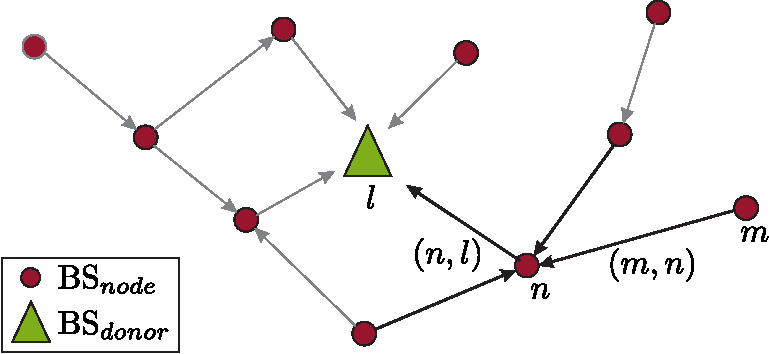
\includegraphics[width=0.6\columnwidth]{Figures/Safehaul/systModelNoWall-eps-converted-to}
      \caption{Example of a graph $\mathcal{G}_i$}
      \label{fig:systModel}
      \vspace{-4mm}
\end{figure}


 Each \node{} $n$ has a finite data buffer with capacity $B^\mathrm{max}_n$ to store the backhaul data to be transmitted to any of the BS-donors. 
 In each time slot $i$, \node{} $n$ is characterized by its load and average queuing time. The load, denoted by $B_{n,i} \in \mathbb{N}$, indicates the number of data packets stored in the buffer at the beginning of time slot $i$. The average queuing time $t^\mathrm{q}_{n,i} \in \mathbb{R}^+$ is the average number of time slots the current packets in the data buffer have been stored.
Additionally, we denote by $M_{n,l,i} \in \mathbb{N}$ the number of data packets transmitted from $n$ and successfully received at $l$ in time slot $i$ (i.e., when $x_{n,l,i}=1$), and with $t^\mathrm{tx}_{n,l,i} \in \mathbb{R^+}$ the transmission time needed to send these packets. Note that $M_{n,l,i}\leq B_{n,i}$ as only packets stored in the data buffer can be transmitted.
At the receiver BS-node $l$, the load $B_{l,i+1}$ of its data buffer is updated at the beginning of the next time slot $i+1$  such that $B_{l,i}+M_{n,l,i}\leq B_l^\mathrm{max}$ holds.
That is to say, packets exceeding the buffer capacity are dropped. Finally, when $x_{n,l,i}=0$ both $M_{n,l,i}$ and $t_{n,l,i}^\mathrm{tx}$ are equal to zero.


We define the maximum tolerable latency $T_\mathrm{max}$ as the maximum time a packet can take from its source \node{} to any BS-donor. Any packet that is not delivered before $T_\mathrm{max}$ milliseconds will be dropped.
 The average maximum end-to-end latency $\bar{T}_{n,d}$ from \node{} $n$ to BS-donor $d$ is the average, over the complete time horizon $I$, of the maximum delay a packet originating from \node{} $n$ takes to reach any BS-donor $d$ in time slot $i$.
This is calculated as $\bar{T}_{n,d} = \frac{1}{I}\sum_{i=1}^I T_{n,d,i}$, 
where $T_{n,d,i}$ is the maximum end-to-end latency among all the packets originating in \node{} $n$ which reach BS-donor $d$ in time slot $i$. 
$T_{n,d,i}$ is a sample of the random variable $T_{n,d}$ drawn from an unknown stationary probability distribution $P$ that depends on the links $x_{n,l,i'}$, $n\in\mathcal{N}$, $l\in{\mathcal{V}}$, $i'=1,\dots,i$, activated up to time $i$, the user's mobility, the location of the \node{} $n$, the interference in the system, and the queue dynamics.
Accordingly, we define the average maximum end-to-end latency in the system $\bar{T}$ as
\begin{equation}
    \bar{T} = \frac{1}{ND}\sum_{n=1}^N\sum_{d=1}^D \bar{T}_{n, N+d}.
    \label{eq:avgDelay}
\end{equation}


 \subsection{Problem Formulation}
\label{s:prob_formulation}
The joint minimization of the average maximum end-to-end latency and the expected value of its tail loss in IAB-enabled networks is formulated in this section. We first introduce \gls{cvar}, the risk metric accounting for minimizing the events in which the end-to-end latency is higher than $T_\mathrm{max}$. Next, we formulate the optimization problem in the complete network.
 
\subsubsection{Preliminaries on CVaR}
Traditionally, latency minimization in IAB-enabled networks has focused on optimizing the expected value of a latency function~\cite{vu2018path, ortiz2019scaros}.
However, such an approach fails to capture the time variability of the latency distribution, thus potentially leading to unreliable systems in which $T_{n,d,i}>T_\mathrm{max}$, for any  $i=1,...,I$, $n\in \mathcal{N}$ and $d\in\mathcal{D}$.
\textit{For this purpose, we consider not only the average end-to-end latency $\bar{T}$ in the system, but also its expected tail loss based on the \gls{cvar}}\cite{Rockafellar2000, Rockafellar2002}.

Having in mind that $T_{n,d}$ is a random variable, we assume it has a bounded mean on a probability space $(\Omega, \mathcal{F}, P)$, with $\Omega$ and  $\mathcal{F}$ being the sample and event space, respectively.
Using a risk level $\alpha\in(0,1]$, the $\mathrm{\gls{cvar}}_\alpha(T_{n,d})$ of $T_{n,d}$ at risk level $\alpha$ quantifies the losses that might be encountered in the $\alpha$-tail. More specifically, it is the expected value of $T_{n,d}$ in its $\alpha$-tail distribution \cite{Rockafellar2002}. 
Formally, $\mathrm{CVaR}_\alpha(T_{n,d})$ is defined as \cite{Rockafellar2000}
\begin{equation}
    \mathrm{CVaR}_\alpha(T_{n,d}) = \min_{q\in\mathbb{R}}\left\{q+\frac{1}{\alpha}\mathbb{E}\left[\max\{T_{n,d}-q,0\}\right]\right\},
    \label{eq:CVaR}
\end{equation}
where the expectation in \eqref{eq:CVaR} is taken over the probability distribution $P$. 
Note that lower $\mathrm{\gls{cvar}}_\alpha(T_{n,d})$ results in higher system reliability because the expected end-to-end latency in the $\alpha$-worst cases is low.
Moreover, note that $\alpha$ is a risk aversion parameter. For $\alpha=1$,  $\mathrm{\gls{cvar}}_\alpha(T_{n,d}) = \mathbb{E}[T_{n,d}]$ which represents the traditional risk-neutral case. 
Conversely, 
$\lim\limits_{\alpha\rightarrow 0}\mathrm{\gls{cvar}}_\alpha(T_{n,d}) = \sup\{T_{n,d}\}$.
\gls{cvar} has been shown to be a coherent risk measure, i.e., it fulfills monotonicity, subadditivity, translation invariance, and positive homogeneity properties \cite{Pflug2000}. 

\subsubsection{Optimization Problem}
We jointly minimize the average maximum end-to-end latency and its expected tail loss for each \node{}. 
For this purpose, we decide which of the $(n,l)$ links to activate in each time slot $i$ during the finite time horizon $I$.
In the following, we formulate the optimization problem from the network perspective and consider the sum over all \nodes{} in the system. 
The latency minimization problem should consider three different aspects: $(i)$ link activation is constrained by the half-duplex nature of self-backhauling, $(ii)$ only data stored in the data buffers can be transmitted, and $(iii)$ packet drop due to buffer overflow should be avoided.
Formally, the problem is written as:


\small{
\begin{minie}[3]
{\{x_{n,l,i} \}}{\sum_{n\in\mathcal{N}}\left(\sum_{d\in\mathcal{D}}\left(\frac{1}{I}\sum_{i=1}^I T_{n,d,i}\right)+\eta\mathrm{\gls{cvar}}_\alpha(T_{n,f})\right) \label{eq:objective}}{\label{eq:OptProblem}}{}
    \addConstraint{\sum_{\substack{l\in\mathcal{V}, l\neq n}} x_{n,l,i}+\sum_{l\in\mathcal{N}}x_{l,n,i}}{=1,\, \label{eq:constHD}}{n\in\mathcal{N}, \, i=1,\dots,I}
    \addConstraint{ B_{n,i}}{\geq  M_{n,l,i,\, \label{eq:constCausal}}}{ n\in\mathcal{N}, l\in\mathcal{V},\, i=1,\dots,I}
    \addConstraint{ B_{l,j} + M_{n,l,j} \label{eq:constOverflow}}{\leq B^\mathrm{max}_l,\,}{ n\in\mathcal{N}, l\in\mathcal{V},\, i=1,\dots,I}
    \addConstraint{x_{n,l,i}}{\in \{0,1\}, }{n\in \mathcal{N}, l\in \mathcal{V},\, i=1,\dots,I.}
\end{minie}
}

\normalsize
In \eqref{eq:objective}, $\eta \in [0,1]$ is a weighing parameter to control the trade-off between minimizing the average maximum end-to-end latency $\bar{T}_{n,d}$ and the expected loss of its tail.
The constraint in \eqref{eq:constHD} considers half-duplex transmissions by ensuring that, in each time slot $i$, every IAB-node communicates with up to one of its neighbors by either receiving or transmitting backhaul data. \eqref{eq:constCausal} considers data causality, i.e., only data already stored in the data buffers can be transmitted, and \eqref{eq:constOverflow} prevents buffer exhaustion.
As the considered scenario is not static, solving \eqref{eq:OptProblem} would require complete non-causal knowledge of the system dynamics during the complete time horizon $I$. However, in practical scenarios, knowledge about the underlying random processes is not available in advance.
For example, the \node{}'s loads $B_{n,i}$ depend not only on the transmitted and received backhaul data, but also on the randomly arriving data from its users. Similarly, the amounts of transmitted data $M_{n,l,i}$ depend on the varying channel conditions of both BS $n$ and $l$. 
As a result, the exact values of $T_{n,l,i}$, $B_{n,i}$ and $M_{n,l,i}$ are not known beforehand.
For this reason, we present in Section \ref{s:algo} \name{}, a multi-agent learning approach to minimize in each \node{} the average maximum end-to-end latency and the expected value of the tail of its loss.
 


 \subsection{Our proposed solution: \name}
\label{s:algo}
In this section, we describe \name{}, a multi-agent learning approach for the joint minimization of the average maximum end-to-end latency and its expected tail loss in IAB mmWave networks. 
In \name{}, each \node{} independently decides which links $(n,l)$ to activate in every time slot $i$ by leveraging a multi-armed bandit formulation. The consensus among the \nodes{} is reached by exploiting the centralized resource coordination and topology management role of \gls{iab}-donors~\cite[Sec. 4.7.1]{3gpp.38.300}. 

\subsubsection{Multi-Armed Bandit Formulation}
Multi-armed bandit is a tool well suited to problems in which an agent makes sequential decisions in an unknown environment\cite{Sutton2018}. 
In our scenario, each \node{} $n$ decides, in each time slot $i$, which of the links $(n,l)$ to activate without requiring prior knowledge about the system dynamics.
The multi-armed bandit problem at \node{} $n$ can be characterized by a set $\mathcal{A}_n$ of actions and a set $\mathcal{R}_n$ of possible rewards. 
The rewards $r_{n,i} \in \mathcal{R}_n$ are obtained in each time slot $i$ as a response to the selected action $a_{n,i} \in \mathcal{A}_n$
and the observed latency. Since every \node{} $n$ selects only one action during each time slot, we enforce the half-duplex constraint in~\eqref{eq:constHD} by defining the set of possible actions as the set of feasible links for \node{} $n$.
In particular, we define $\mathcal{A}_n$ for $n \in \mathcal{N}$ as $\mathcal{A}_{n} = \{(n,l), (m,n)| m\in \mathcal{N}, \,l\in\mathcal{V} \}$,
where link $(n,n)$ indicates that \node{} $n$ remains idle.
As blockages, overloads, or failures might render certain links $(n,l)$ temporarily unavailable, we define the set $\mathcal{A}_{n,i} \subseteq \mathcal{A}_n$ of available actions  in time slot $i$ as $\mathcal{A}_{n,i} = \{(n,l), (l,n)|(n,l), (l,n) \in \mathcal{E}_i \}$.
Selecting action $a_i=(n,l)$ in time slot $i$ implies $x_{n,l,i}=1$.

The rewards $r_{n,i}$ are a function of the end-to-end latencies ${T}_{n,d,i}$ and depend on whether at \node{} $n$ a link $(n,l)$ or $(l,n)$ is activated. 
\node{} $n$ is connected to the \donor{} via multi-hop wireless links. 
Consequently, $T_{n,d,i}$ cannot be immediately observed when a link $(n,l)$,  with $l \notin \mathcal{D}$ is activated.
In fact, the destination \donor{} $d$ might not even be known to \node{} $n$ in time slot $i$.
To overcome this limitation, we define the rewards $r_{n,i}$ as a function of the next-hop's estimated end-to-end latency $\hat{T}_{l,d,i}$ as
\begin{equation}
r_{n,i}=\begin{cases}
t^\mathrm{q}_{l,i} + t^\mathrm{tx}_{n,l,i} + \hat{T}_{l,d,i}, &\text{for link } (n,l) \\
t^\mathrm{q}_{n,i} + \hat{T}_{n,d,i}, & \text{for link } (l,n),
\end{cases}
\label{eq:rewards}
\end{equation}
where $\hat{T}_{l,d,i}$ is calculated as $\hat{T}_{l,d,i} = \underset{(l,m) \in \mathcal{E}_i}{\min}\;\hat{T}_{l,m,i}$ and $t_{n,l,i}^\mathrm{tx}$ is calculated based on $M_{n,l,i}$ to ensure the causality constraint in (3c) is fulfilled. Note that the constraint in (3d) cannot be enforced, since multi-armed bandit algorithms learn from the activation of both optimal and suboptimal links.



\subsubsection{Latency and CVaR Estimation}
As given in \eqref{eq:rewards}, \node{} $n$ learns which links $(n,l)$ to activate by building estimates of the expected latency $\hat{T}_{n,l}$ associated to each of them.
Let $K_{n,l,i}=\sum_{j=1}^i x_{n,l,i}$ be the number of times link $(n,l)$ has been activated up to time slot $i$. The estimated $\hat{T}_{n,l}$ is updated using the sample mean as 
\begin{equation}
    \hat{T}_{n,l,i+1} = \frac{K_{n,l,i}\hat{T}_{n,l,i} + r_{n,i}}{K_{n,l,i}+1},
    \label{eq:delayEstimateSM}
\end{equation}
where the subindex $i$ is introduced to emphasize that the estimate is built over time.


The \gls{cvar} definition given in \eqref{eq:CVaR} requires $T_{n,d}$ which, as discussed before, is not known a priori. 
Hence, we leverage the \gls{cvar} estimator derived in \cite{Luo2017} to calculate the estimated \gls{cvar} of a link $(n,l)$. Let  $\Tilde{r}_n^1,\dots,\Tilde{r}_n^{K_{n,l,i}}$ be all the rewards received up to time $i$.
The estimated $\widehat{\mathrm{\gls{cvar}}}_i(n,l)$ in time slot $i$ is calculated as \cite{Luo2017}
\begin{equation}
    \widehat{\mathrm{\gls{cvar}}}_i(n,l) := \inf_{t \in \mathbb{R}}\left(t + \frac{1}{\alpha \cdot K_{n,l,i}}\sum_{k=1}^{K_{n,l,i}}[\Tilde{r}^k_{n} - t]^+\right). 
    \label{eq:cvarEstimate}
\end{equation}




Using the estimates in \eqref{eq:delayEstimateSM} and \eqref{eq:cvarEstimate}, \node{} $n$ computes the value $Q_n(a_{n,i}=(n,l))$ associated to the selected action $a_n\in \mathcal{A}_n$, and defined as
\begin{equation}
    Q_n(a_{n,i})=\hat{T}_{n.l,i} + \eta \widehat{\mathrm{\gls{cvar}}}_i(n,l).
    \label{eq:Qvalue}
\end{equation}
Note that \eqref{eq:Qvalue} is aligned with the objective function in \eqref{eq:objective}. Actions with an associated low value $Q_n(a_{n,i})$ lead to lower end-to-end latency and a low expected value on its tail. 



\subsubsection{Consensus}
\label{s:consensus}
All the \nodes{} independently decide which links to activate based on their estimates of the end-to-end latency. 
As a consequence, conflicting actions may be encountered. 
A conflict occurs when two or more \nodes{} $n$ and $m$ aim at activating a link to a common BS $l$, $l \in \mathcal{V}$, i.e., $x_{n,l,i}=x_{m,l,i}=1$.
We reach consensus by first retrieving the buffer and congestion status of the various \gls{iab}-nodes, leveraging the related \gls{bap} layer functionality~\cite[Sec. 4.7.3]{3gpp.38.300}.
With this information at hand, conflicts are resolved by prioritizing the transmission of the \node{} with the larger queuing times $t^\mathrm{q}_{n,i}$ and loads $B_{n,i}$.
Then, we let the \gls{iab}-donor mark as \textit{unavailable} the time resources of the remaining base stations with conflicting scheduling decisions~\cite[Sec. 10.9]{3gpp.38.300}.
Note that as the learning is performed at each \node{}, only the link activation decision and the weighted sum of $t^\mathrm{q}_{n,i}$ and $B_{n,i}$ are transmitted.
Thus, low communication overhead is achieved.

\subsubsection{Implementation of \name{}}
Here, we describe how the above-mentioned solution can be implemented in a real system. Specifically, we elaborate on the required inputs and the interactions among the different entities as well as the pseudo-code of \name{}, see Alg. \ref{alg:algo}. 

\name{} is executed at each \node{} $n$. For its implementation, the \gls{mno} provides $\alpha$, $\eta$ and $\mathcal{A}_n$ as an input. $\alpha$ is the risk level parameter that influences the level of reliability achieved in the system. Similarly, $\eta$ controls the impact of the minimization of the latency in the $\alpha$-worst cases on the overall performance. Both parameters, $\alpha$ and $\eta$, are set by the \gls{mno} depending on its own reliability requirements.
The set $\mathcal{A}_n$ depends on the considered network topology, which is perfectly known by the \gls{mno}. $\mathcal{A}_n$ includes all links $(n,l)$ and $(l,n)$ to and from the first-hop neighbors of \node{} $n$.
\begin{algorithm}[t]
\footnotesize
\begin{algorithmic}[1]
    \Require $\alpha$, $\eta$, $\mathcal{A}_n$
    \State Initialize $\hat{T}_{n,l}$, $\widehat{\mathrm{\gls{cvar}}}(n,l)$, and $Q_n$ for all $(n,l) \in \mathcal{E}_1$ \label{line:initEst}
    \State Set counters $K_{n,l}=0$ and initial action $a_{n,1}=(n,n)$ \label{line:initCounter}
	\For {every time slot $i=1,...,I$}
	    \State perform action $a_{n,i}$, observe reward $r_{n,i}$ and increase counter $K_{n,l}$ by one \Comment{Eq. \eqref{eq:rewards}} \label{line:reward}
\State update latency estimate $\hat{T}_{n,l}$ \Comment{Eq: \eqref{eq:delayEstimateSM}} \label{line:updateEstDelay}
		\State update \gls{cvar} estimate $\widehat{\mathrm{\gls{cvar}}}(n,l)$ \Comment{Eq: \eqref{eq:cvarEstimate}} \label{line:updateCvar}
		\State update $Q_n(a_{n,i})$ \Comment{Eq: \eqref{eq:Qvalue}} \label{line:updateQ}
		\State select next action $a_{n,i+1}$ using $\epsilon$-greedy \Comment{Eq. \eqref{eq:epsGreedy}} \label{line:epsGreedy}
		\State share $a_{n,i+1}$, $t^\mathrm{q}_{n,i}$ and $B_{n,i}$ with the other \nodes{} \label{line:share}
		\State if required, update $a_{n,i+1}$ to reach consensus \Comment{Section \ref{s:consensus}} \label{line:consensus}
\EndFor
\end{algorithmic}
\caption{\name{} algorithm at each \node{}} \label{alg:algo} 
\end{algorithm}

The execution of \name{} begins with the initialization of the latency and \gls{cvar} estimates, and the values $Q$ of the actions in $\mathcal{A}_n$.
Additionally, the counters $K_{n,l}$, that support the calculations of $\hat{T}_{n,l}$ and $\widehat{\mathrm{\gls{cvar}}}(n,l)$, are initialized for all links in $\mathcal{A}_n$ (lines \ref{line:initEst}-\ref{line:initCounter}).
These parameters are updated and learnt throughout the execution of \name{}.
At time slot $t=0$, no transmission has occurred and $B_{n,0}=0$. Hence, \node{} $n$ remains idle for the first time slot $i=1$, i.e., $a_{n,1}=(n,n)$ (line \ref{line:initCounter}).
Next, and in each of the subsequent time slots $i\in \{1,\ldots, I\} $, the selected action is performed and the corresponding reward is obtained (line \ref{line:reward}).
If \node{} $n$ transmits in time slot $i$, i.e., $a_{n,i}=(n,l)$, the reward $r_{n,i}$ is sent by the receiving BS $l$ through the control channel.
If $a_{n,i}=(l,n)$, the reward $r_{n,i}$ depends, as given in \eqref{eq:rewards}, only on the current estimates at \node{} $n$ and the status of its buffer $B_{n,i}$.
With the observed reward $r_{n,i}$, the counter for action $a_{n,i}$ is increased and the latency and \gls{cvar} estimates are updated (lines \ref{line:reward}-\ref{line:updateCvar}).
Using the new estimates (lines \ref{line:updateEstDelay} and $\ref{line:updateCvar}$), the value $Q(a_{n,i})$ of the performed action $a_{n,i}$ is updated (line \ref{line:updateQ}).
The next action $a_{n,i+1}$ is then selected according to $\epsilon$-greedy (line \ref{line:epsGreedy}), which is a well-known method to balance the exploitation of links with estimated low latency, and the exploration of unknown but potentially better ones.
In $\epsilon$-greedy, a random action $a_{n,i+1}$ from the set $\mathcal{A}_{n,i+1}$ is selected with probability $\epsilon \in [0,1]$.
With probability $(1-\epsilon)$, instead, the action that yields the estimated lowest value is chosen, i.e., 
\begin{equation}
a_{n,i+1} = \begin{cases}
\text{randomly selected action from } \mathcal{A}_{n,i+1}, & \text{if } x\leq\epsilon \\
\underset{b_n \in \mathcal{A}_{n,i+1}}{\argmax} \, Q_n(b_{n}), & \text{if } x>\epsilon, 
\end{cases}
    \label{eq:epsGreedy}
\end{equation}
where $x$ is a sample taken from a uniform distribution in the interval $[0,1]$.
Once the action $a_{n,i+1}$ is selected, it is shared with other \nodes{} in the network along with $t^\mathrm{q}_{n,i}$ and $B_{n,i}$ (line \ref{line:share}).
As described in Section~\ref{s:consensus}, this goes through the control channel. 
If conflicts arise, consensus is reached by prioritizing the transmission of the \node{} with the largest loads and queuing times (line \ref{line:consensus}).

\subsubsection{Regret Analysis}
The regret $\zeta$ is defined as the expected loss caused by the fact that the optimal action is not always selected \cite{Auer2002}. 
Let $\bar{T}^*$ and $\Bar{T}_{a_n}$ be the expected delay associated to the optimal action $a^* \in \mathcal{A}_n$ and the non-optimal action $a_n \in \mathcal{A}_n$, respectively. Similarly, let $\mathrm{\gls{cvar}}^*$ and $\mathrm{\gls{cvar}}_{a_n}$ be the \gls{cvar} of the optimal action $a^* \in \mathcal{A}_n$ and the non-optimal action $a_n\in \mathcal{A}_n$, respectively.
Formally, the regret $\zeta_i$ after $i$ time slots is defined as
\begin{align}
\label{eq:regret}
    \zeta_i &=\!\! \sum_{a_n \in \mathcal{A}_n}\!\left( \left(\Bar{T}_{a_n} + \eta\mathrm{\gls{cvar}}_{a_n}\right) - \left(\Bar{T}^* + \eta\mathrm{\gls{cvar}}^*\right)\right)\mathbb{E}[K_{a_n,i}]  \nonumber \\
    &= \!\! \sum_{a_n \in \mathcal{A}_n}\Delta_{a_n}\mathbb{E}[K_{a_n,i}], 
\end{align}
where $K_{a_n,i}$ is the number of times action $a_n$ has been selected up to time slot $i$.

\begin{proposition}
\label{prop:probNonOptArm}
For a network $\mathcal{G}$ in which the independent decisions of the \nodes{} do not lead to conflicts, let
$A_n=|\mathcal{A}_n|$ be the number of available actions for \node{} $n$. Additionally, let $c > 0$, $0 < d \leq 1$, and $\epsilon_i := \min(1, \frac{cA_n}{d^2i})$.
Then, there exists a positive constant $C > 1$, such that the probability that \name{} chooses a non-optimal action $a_n \neq a^*$ after $i\geq cA_n/{d}$ time slots is upper bounded as
\begin{align*}
\mathbb{P}[a_{n,i} = a_n] \leq & \frac{c}{d^2i} + \frac{4e}{d^2}B_i^{\frac{c}{2}} + \frac{2Cd^2}{c \mathrm{ln}\left(\frac{(i-1)d^2e^{0.5}}{cA_n}\right)} \\
    & + 4C\left(\frac{c}{d^2}\mathrm{ln}\left(\frac{(i-1)d^2e^{0.5}}{c A_n}\right)\right) B_i^{\frac{c}{5d^2}},
\end{align*}
with $B_i = \frac{c A_n}{(i-1)d^2e^{0.5}}.$
\end{proposition}
\begin{proof}
See the Appendix.
\end{proof}

\begin{theorem}
\label{theo:regret}
For a network $\mathcal{G}$ in which the independent decisions of the \nodes{} do not lead to conflicts, the regret $\zeta_i$ of \name{} after $i$ time slots is upper bounded by
\begin{align*}
    \zeta_i \leq \!\!\sum_{a_n\in \mathcal{A}_n} & \!\!\Delta_{a_n} \!\!\left(1+\sum_{i'=2}^i\left[ \frac{c}{d^2i'} + \frac{4e}{d^2}B_{i'}^{\frac{c}{2}} +  \frac{2Cd^2}{c \mathrm{ln}\left(\frac{(i'-1)d^2e^{0.5}}{cA_n}\right)}\right.\right. \\ 
    & + \left.\left. 4C\left(\frac{c}{d^2}\mathrm{ln}\left(\frac{(i'-1)d^2e^{0.5}}{c A_n}\right)\right) B_{i'}^{\frac{c}{5d^2}} \right]\right),
\end{align*}
where 
$c > 0$ and $0 < d \leq 1$.
\end{theorem}

\begin{proof}
From the definition in \eqref{eq:regret}, the regret can be upper bounded as 
\begin{equation}
\zeta_i \leq \sum_{a_n\in\mathcal{A}_n}{\Delta_{a_n} \left(1+\sum_{i'=2}^i\mathbb{P}[a_{n,i'}=a_n]\right)} \label{eq:regret2},
\end{equation}
by considering that $\mathbb{E}[K_{a_n,i}]\leq 1+\sum_{i'=2}^i\mathbb{P}[a_{n,i'}=a_n]$. 
The bound is obtained by including the result of Proposition \ref{prop:probNonOptArm} in \eqref{eq:regret2} as
\begin{align}
    \zeta_i \leq \!\!\sum_{a_n\in \mathcal{A}_n} & \!\! \Delta_{a_n}\!\! \left(1+\sum_{i'=2}^i\left[ \frac{c}{d^2i'} + \frac{4e}{d^2}B_{i'}^{\frac{c}{2}}  + \frac{2Cd^2}{c \mathrm{ln}\left(\frac{(i'-1)d^2e^{0.5}}{cA_n}\right)}
    \right.\right. \nonumber \\
    &+ \left.\left. 4C\left(\frac{c}{d^2}\mathrm{ln}\left(\frac{(i'-1)d^2e^{0.5}}{c A_n}\right)\right) B_{i'}^{\frac{c}{5d^2}}  \right]\right),
\end{align}
As every term in square brackets decreases monotonically in $i'$, the regret $\zeta_i$ grows sub-linearly.

\end{proof}  

\subsection{Simulation setup}
\label{s:simulation_setup}
Given the lack of access to actual 5G (and beyond) network deployments, prior works mostly rely on \textit{home-grown} simulators for performance evaluation. Although this is a valid approach, these simulators often cannot fully capture the real network dynamics, introducing strong assumptions in the physical and/or the upper layers of the protocol stack. 
Until very recently, the most complete  simulator for \gls{iab} networks was a system-level simulator~\cite{8514996} developed as an extension of the ns-3 \textit{mmWave} module~\cite{8344116}. However, despite accurate modeling of the \gls{iab} protocol stack, it is currently behind the latest \gls{iab} specifications\footnote{For instance due to the assumption of L-3 (instead of L-2) relaying at the \gls{iab}-nodes which was based on a draft version of TR 38.874~\cite{3gpp_38_874_old}.}. Moreover, the ns-3 \gls{iab} extension is unsuitable for large simulations with hundreds of nodes due to reliance on an older version of the \textit{mmWave} module. Therefore, in our work we opt for Sionna~\cite{hoydis2022sionna}, which is an open-source GPU-accelerated toolkit based on TensorFlow. 

However, unlike the aforementioned ns-3 module, Sionna is a physical layer-focused simulator that does not explicitly model 5G networks, thus lacking  the characterization of the 5G-NR upper-layer protocol stack. Hence, we extend Sionna by including the system-level functionalities such as MAC-level scheduling and RLC-level buffering. Furthermore, since Sionna exhibits slight differences compared to the 5G-NR physical layer, we extend Sionna's physical layer model~\cite{hoydis2022sionna} with the 5G-NR procedures. In the following, we describe the details of our extensions, which are publicly available\footnote{\url{https://github.com/TUDA-wise/safehaul_infocom2023}}.


\begin{figure}[t!]
    \centering
    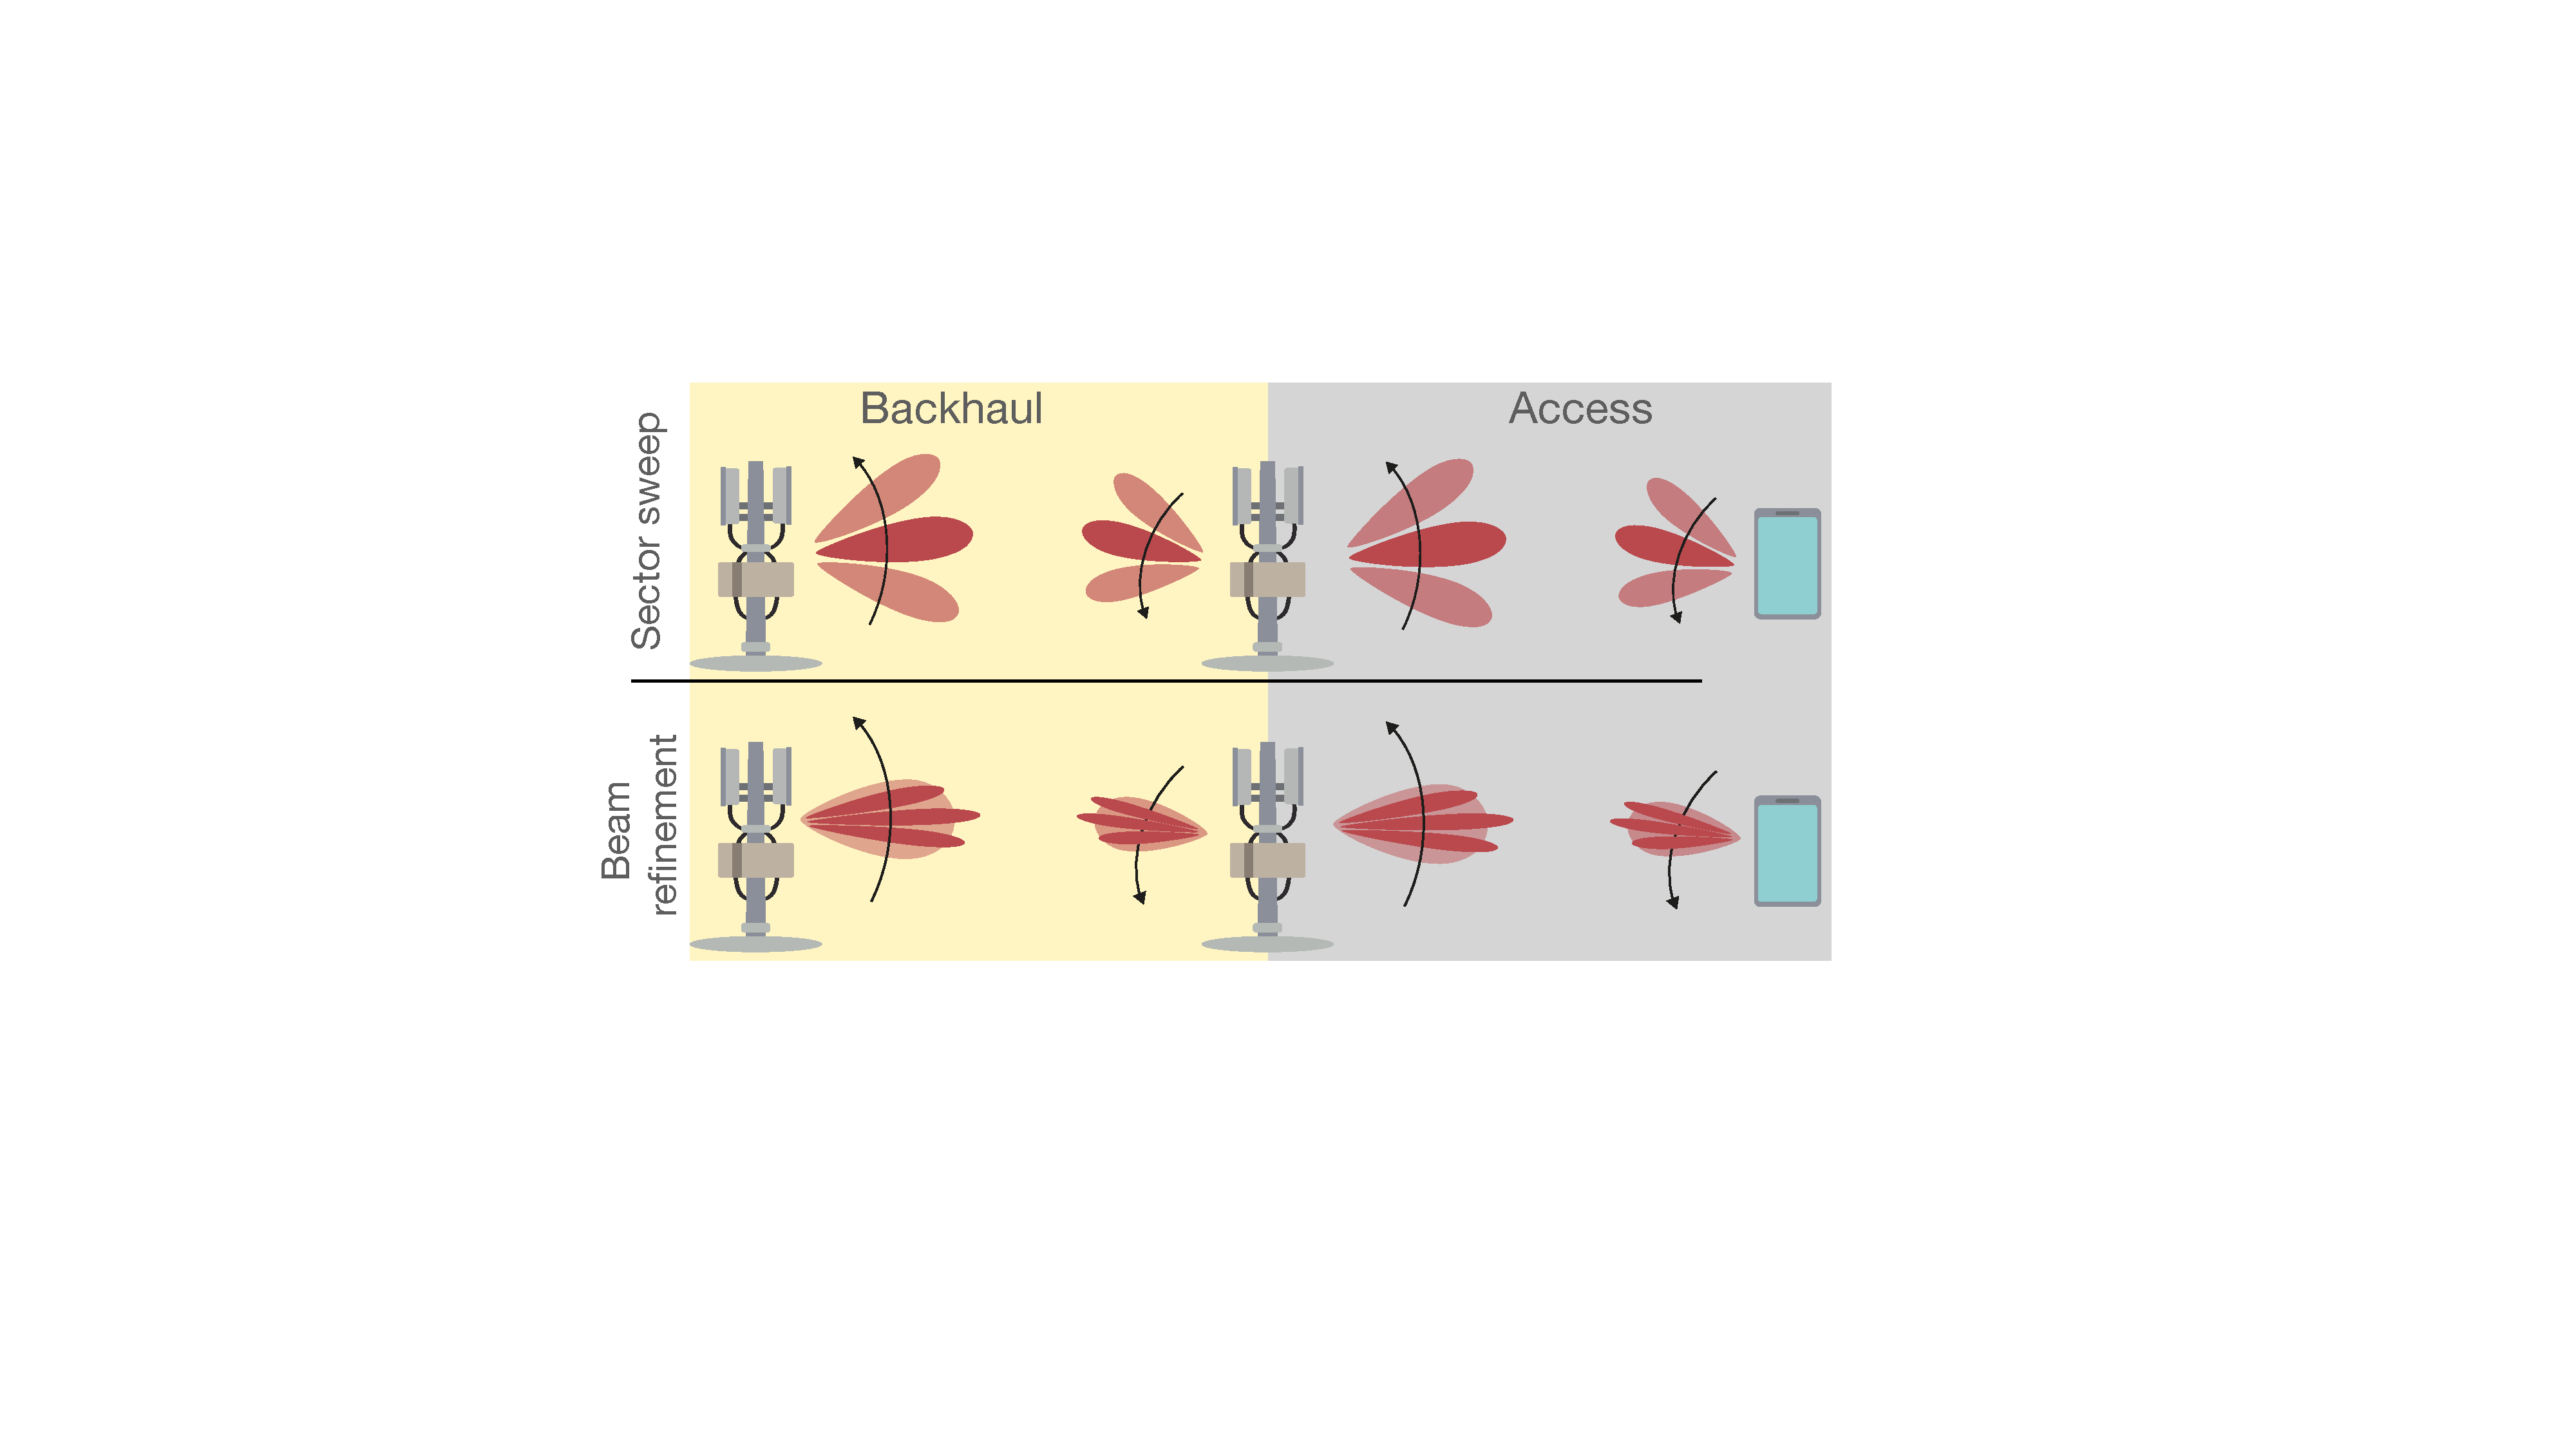
\includegraphics[scale=0.28]{Figures/Safehaul/Beamforming-2.pdf}
      \caption{Schematic of the hierarchical beam management procedure. First, the general direction is estimated using wide beams (top). Then, the search is refined using the narrow beams codebook.}
      \label{fig:beamforming}
      \vspace{-5mm}
\end{figure}



\subsubsection{Extensions to Sionna's physical layer module}
\label{sub:additionalSionna}
In this section, we describe the physical layer modification that were necessary to evaluate IAB scenarios using Sionna. 

\paragraph{Codebook-based Beamforming}
Sionna's native beamforming only supports \gls{zf} pre-coding in downlink. Therefore, as a first step, we extend Sionna by implementing an NR-like codebook-based analog beamforming both at the transmitter and at the receiver.
Specifically, we assume that the beamforming vectors at the transmitter $w_{tx}$ and at the receiver $w_{rx}$ are a pair of codewords selected from a predefined codebook. The codebook is computed by defining a set of beam directions $\{ \omega_{p,q} \}$ which scans a given angular sector with a fixed beamwidth. The steering vector $a_{p,q}$ corresponding to direction $\omega_{p, q}$ can be computed as:
\medmuskip=1mu
\thinmuskip=1mu
\thickmuskip=1mu
\begin{equation}
    \begin{aligned}
            a_{p,q} &= \left[ 1,\ldots, e^{j\frac{2\pi}{\lambda}d\left(i_{ H}\sin\alpha_p\sin\beta_q+i_{V}\cos\beta_q\right)}, \ldots,  \right. \\ 
            & \left. e^{j\frac{2\pi}{\lambda}d\left((N_{H}-1)\sin\alpha_p\sin\beta_q + (N_{ V}-1)\cos\beta_q\right)} \right] ^T,
    \end{aligned}
\end{equation}
\medmuskip=6mu
\thinmuskip=6mu
\thickmuskip=6mu
where $N_{H}$ and $N_{V}$ are the number of horizontal and vertical antenna elements, respectively. The horizontal and vertical indices of a radiating element are denoted by $i_{H}\in \{0, \ldots, N_{H} - 1 \}$ and $i_{V}\in \{0, \ldots, N_{V} - 1\}$, respectively. $\alpha_p$ and $\beta_q$ represent the azimuth and elevation angles of $\omega_{p, q}$. Next, we define the codebook as the set $\{ \left( \sqrt{N_{H} N_{V}} \right)^{-1} w_{p, q} \}$. 

In line with the 5G-NR beam management procedure~\cite{giordani2018tutorial}, we assume the lack of complete channel knowledge, i.e., the communication endpoints do not know the corresponding channel matrix. Accordingly, an exhaustive search is conducted to identify the best pair of codewords resulting in the highest \gls{sinr}. We leverage a hierarchical search, in which the communication pairs first perform a wide-beam search
in which the transmitter and the receiver approximate the direction of communication, see Figure~\ref{fig:beamforming}. Next, the beamforming direction is fine-tuned through a beam refinement procedure going through a codebook with narrow beams. Consequently, we employ two types of codebooks, one with wide beams for sector sweep and another with narrow beams for beam refinement.   

\paragraph{SINR Computations}

Since Sionna does not natively calculate the \gls{sinr}, we add this functionality to the simulator to better model the impact of interference in our simulations. We compute the \gls{sinr} experienced by \glspl{tb} by combining the power of the intended signal with that of the interferers and of the thermal noise. Specifically, we first compute the power $P_{n}(i,f)$ of the intended signal at receiver $n$ over frequency $f$ and in time slot $i$. Then, we obtain the overall interference power by leveraging the superposition principle and summing the received power from all other interfering base stations $P_{m} (i, f)$ where $m \neq n$. For the purposes of this computation, we assume that each interferer employs the beamforming vector yielding the highest \gls{snr} towards its intended destination. Similarly, the transmitter and the receiver use the beamforming configuration estimated via the hierarchical search procedure. Finally, the \gls{sinr} is 
\begin{equation}
    \label{EQ_CGAN1}
    \gamma_{n} (i, f)= \frac{P_{n}(i,f)}{\sum\limits_{m \neq n} P_{m}(i,f) + \sigma^2(i,f)} ,
\end{equation}
where $\sigma^2(i,f)$ is the thermal noise power at the receiver.

\begin{figure}
\centering
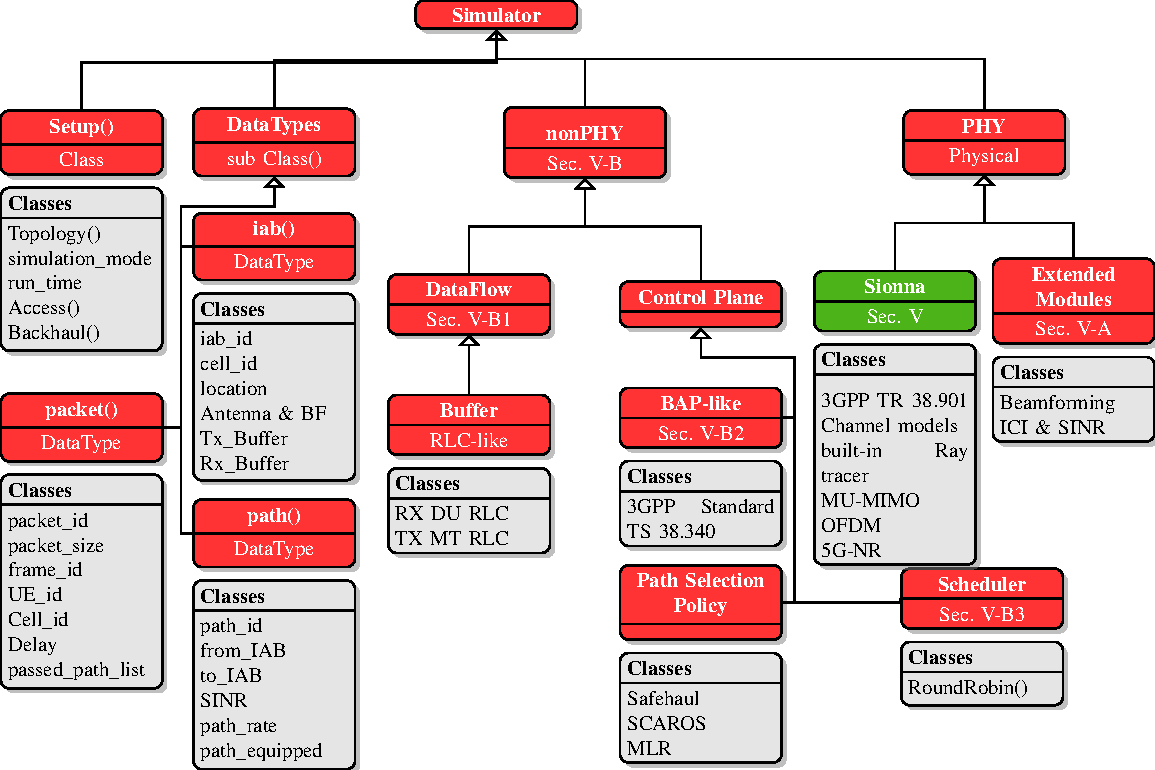
\includegraphics[width=0.85\textwidth]{Figures/Safehaul/simulator_diagram.pdf}
\caption{Overall design of our Sionna's extension. The red blocks represent our additions to the baseline simulator, i.e., Sionna~\cite{hoydis2022sionna}.}
\label{fig:simulator_design}
\end{figure}

As mentioned, Sionna is mainly a physical layer simulator. However, to get closer to \gls{iab} networks as specified in Rel. 17, we have extended Sionna by implementing a selection of system-level features. To such end, we introduced a discrete-event network simulator for modeling \gls{iab} networks. This system-level extension operates on top of Sionna and provides basic functionalities such as a \gls{mac}-level scheduler, layer-2 buffers, and data flow and path selection mechanisms. Our simulator, depicted in Figure~\ref{fig:simulator_design}, generates a variety of system-level KPIs such as latency, throughput, and packet drop rate. 


\paragraph{Data Flow and buffer}
\label{sub:Dataflow}
3GPP has opted for a layer-2 relaying architecture for \nodes{} where hop-by-hop \gls{rlc} channels are established. This enables retransmissions to take place on the affected hops only, thus preventing the need for traversing again the whole route from the \donor{} whenever a physical layer \gls{tb} cannot be successfully decoded. This design results in a more efficient recovery from transmission failures and reduces buffering at the communication endpoints~\cite{madapatha2020integrated}. To mimic this architecture, we have implemented RLC-like buffers at each base station. Specifically, each \node{} features layer-2 buffers for both received and transmitted packets.
For instance, the data flow for an uplink packet is the following.
The \gls{ue} generates packets and sends a transmission request to the base station. Consequently, the scheduler allocates OFDM symbols for this transmission, which is eventually received and stored at the RX buffer of its \gls{du}. Next, the packet is placed into the TX buffer to be forwarded to the suitable next hop \node{}. This procedure is repeated until the packet crosses all the wireless-backhaul hops and reaches the \donor. Note that the packet can be dropped due to latency constraints or to interference.

\paragraph{\gls{bap}}
\label{sub:bap}
To manage routing within the wireless-backhauled network, the 3GPP introduced \gls{bap}, i.e., an adaptation layer above \gls{rlc} which is responsible for packet forwarding between the \donor{} and the access \nodes~\cite{3gpp_38_340}. Our simulator mimics this by associating each \node{} to a unique \gls{bap} ID. Moreover, we append a \gls{bap} routing ID to each packet at its entry point in the \gls{ran} (i.e., the \donor{} and the \glspl{ue} for DL and UL data, respectively).  Then, this identifier is used to discern the (possibly multiple) routes toward the packet's intended destination~\cite{3gpp_38_340}. The choice of the specific route is managed by \name{}.


\paragraph{Scheduler}
\label{sub:scheduler}
Finally, we implemented a \gls{mac}-level scheduler which operates in a \gls{tdma} mode. The scheduler periodically allocates the time resources to backhaul or access transmissions in a Round-Robin fashion\footnote{The choice of the specific scheduling algorithm is outside of the scope of the 3GPP NR specifications, and is thus left to the MNOs. Accordingly, a Round-Robin scheduling policy represents a typical baseline assumption.}. Specifically, each cell first estimates the number of OFDM symbols needed by each data flow by examining the corresponding buffer. Then, the subframe's OFDM symbols are equally allocated to the users. If a user requires fewer symbols to transmit its complete buffer, the excess symbols (the difference between the available slot length and the needed slot length) are distributed to the other active users. 

\subsection {Performance Evaluation}
\label{s:simulation_analysis}

\begin{figure}
    \centering
    \subfloat[][Manhattan (223 \nodes{}).]{
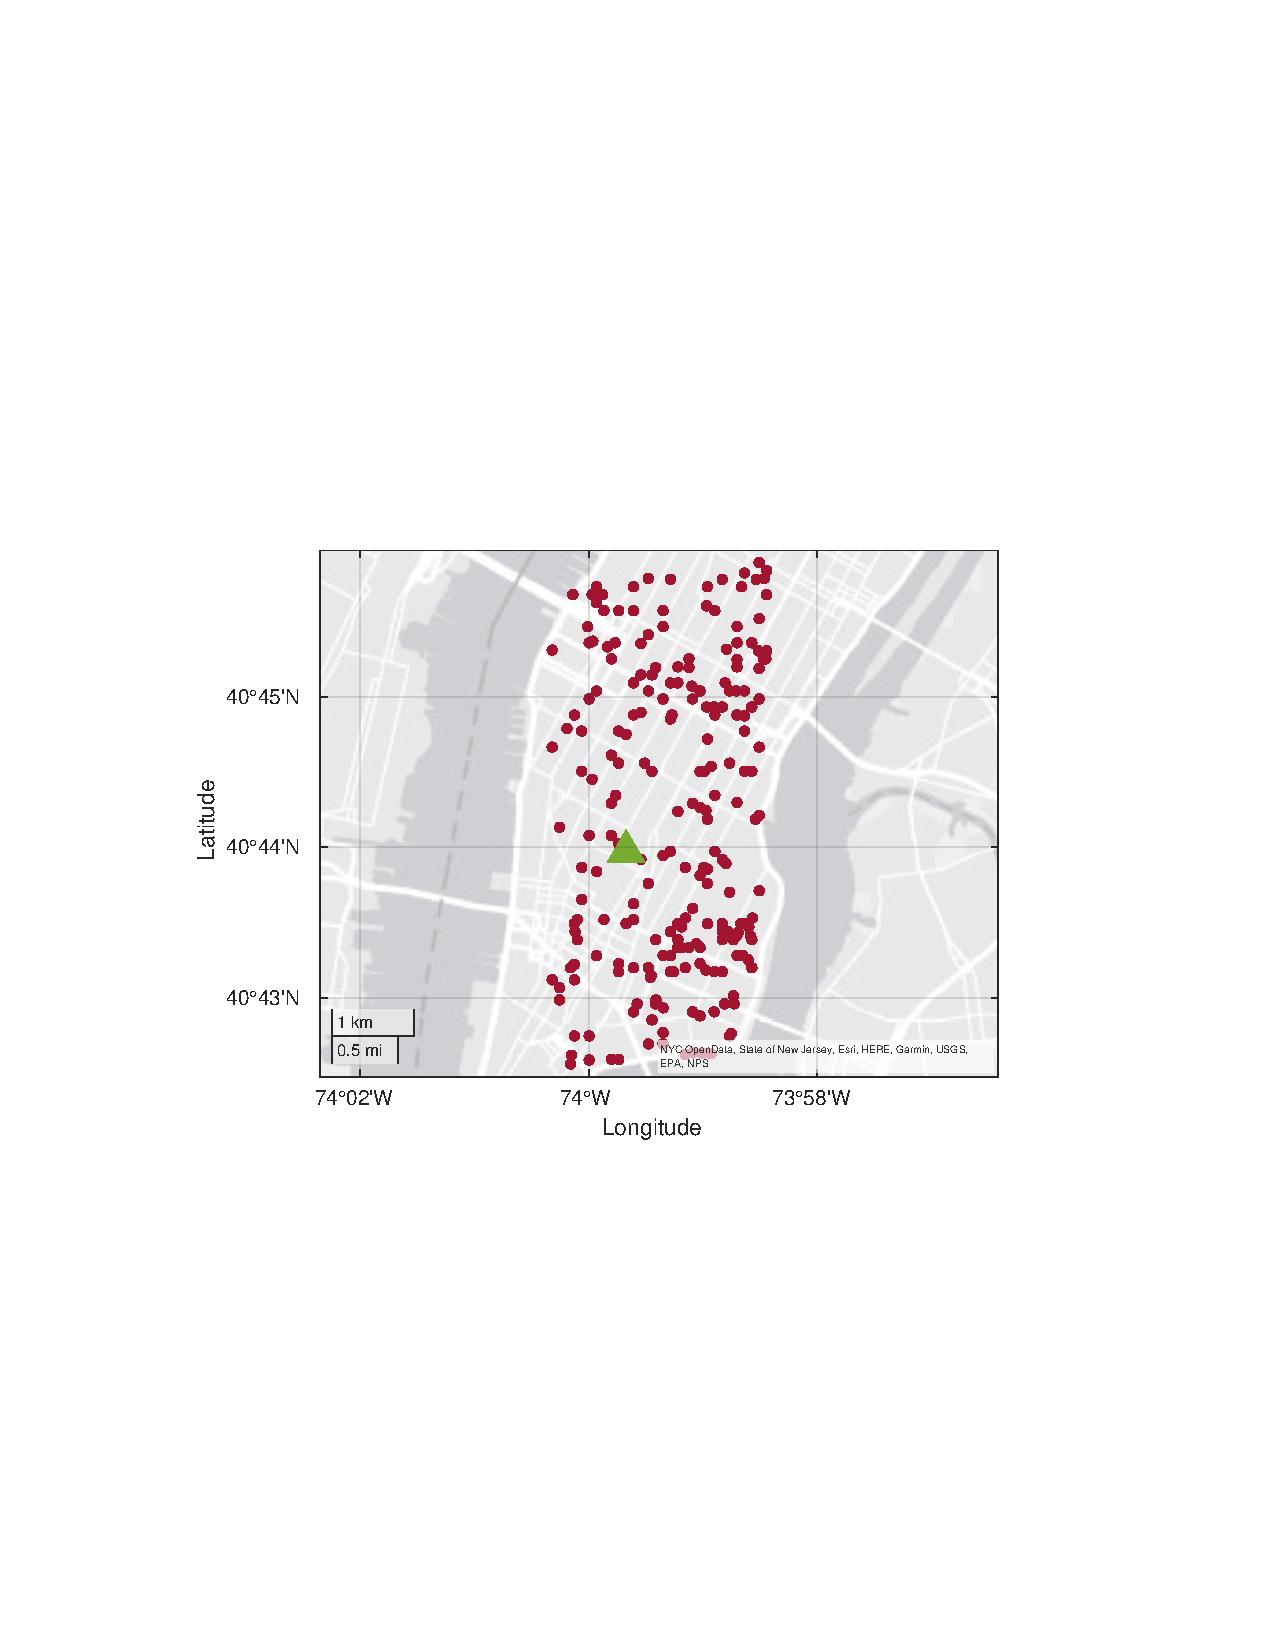
\includegraphics[scale=0.45]{Figures/Safehaul/manhattan_new.pdf}
    \label{fig:manhattan}}
    \subfloat[][Padova (100 \nodes{}).]{
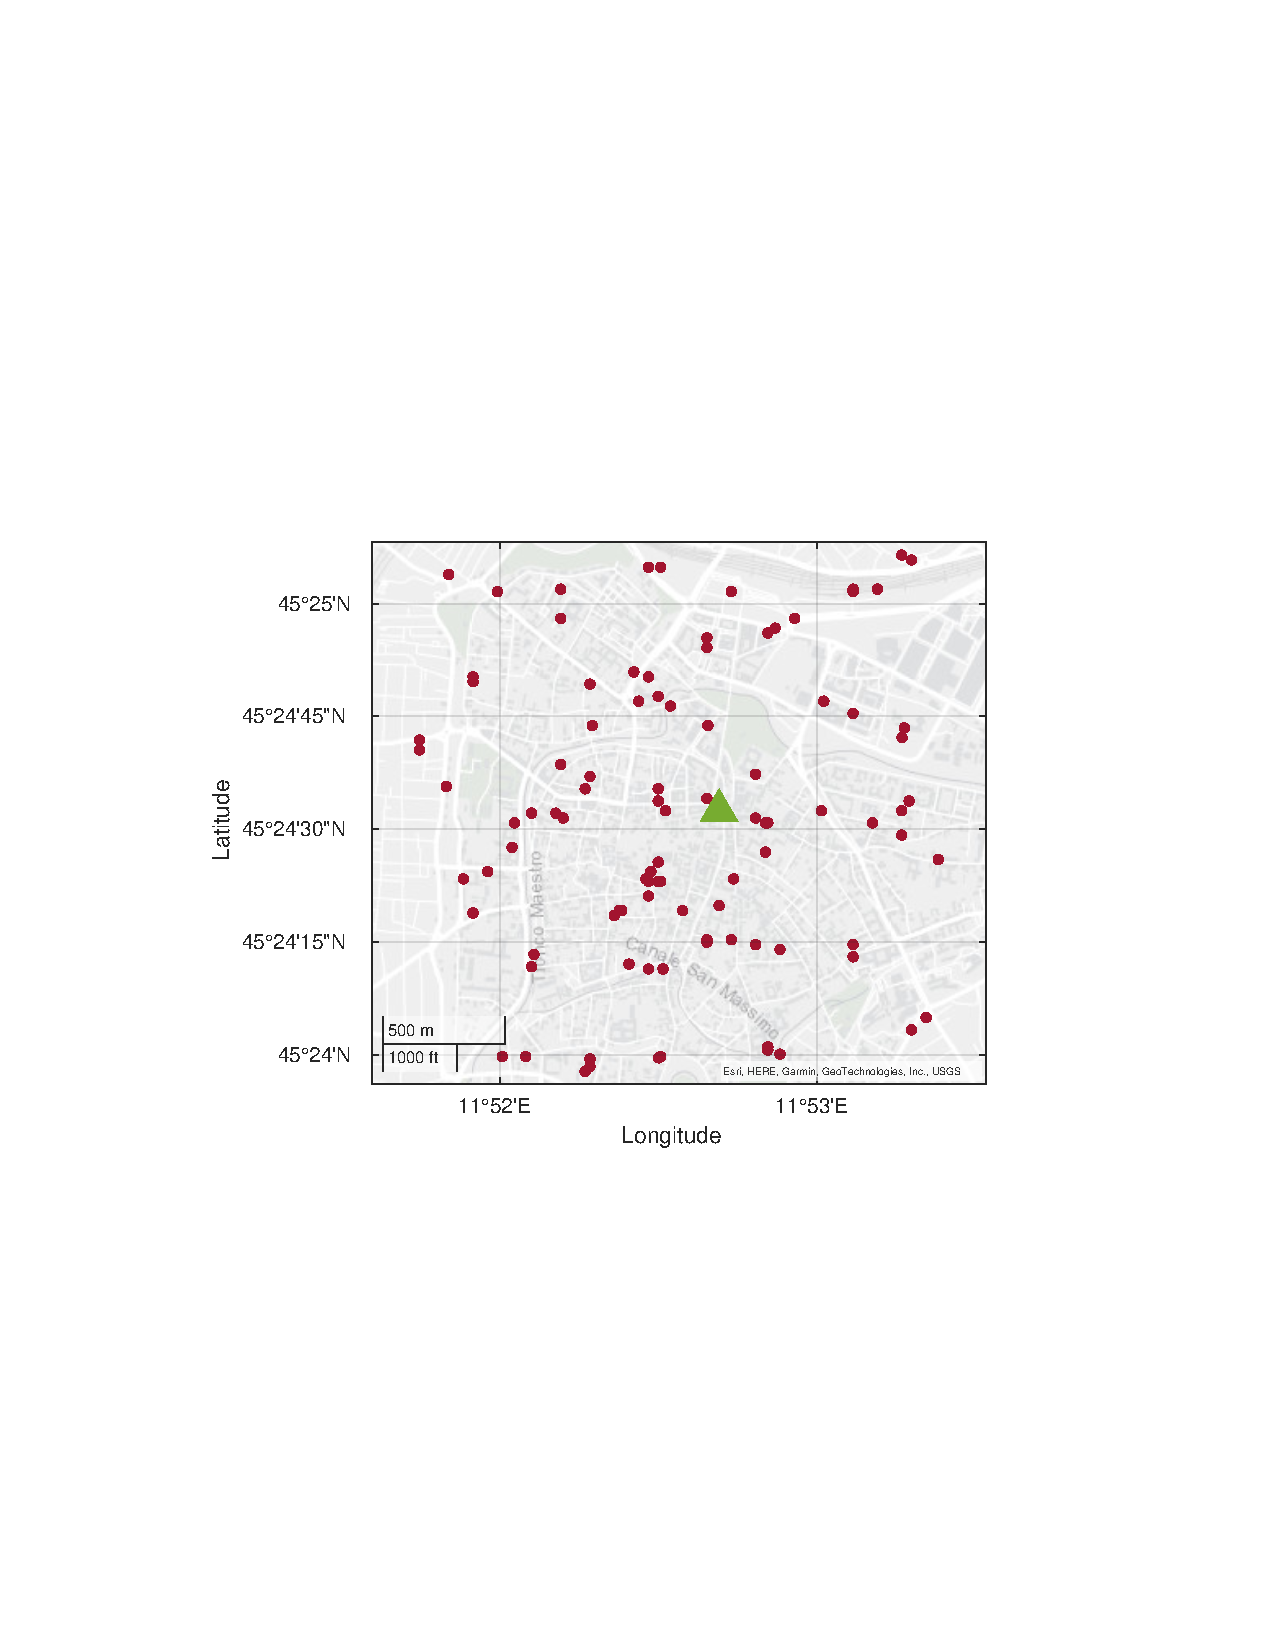
\includegraphics[scale=0.45]{Figures/Safehaul/padova_new.pdf}
    \label{fig:Padova_Map}}
    \caption{Locations of \nodes{} (red dots) and of the \donor{} (green triangle) in the Manhattan (left) and Padova (right) topologies.}
\end{figure}


\begin{figure*}[t!]
\centering
\subfloat[][Average per-UE end-to-end latency]{
    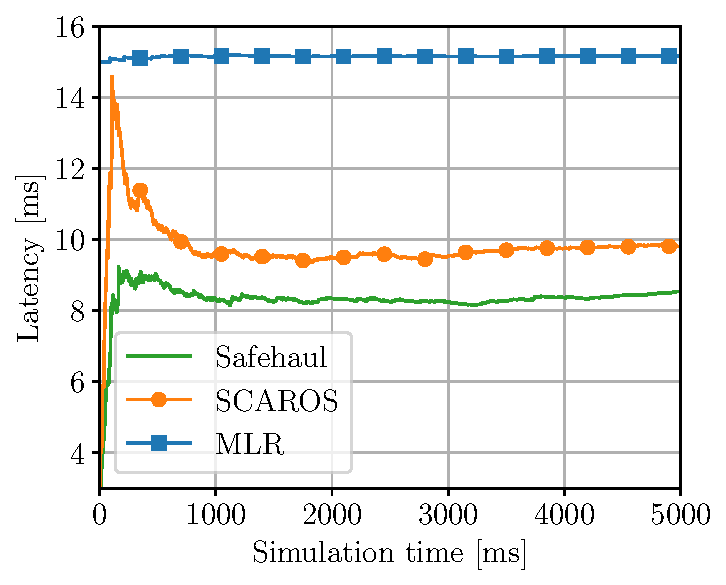
\includegraphics[width=.45\linewidth]{Figures/Safehaul/S1_lat_vs_time.pdf}
    \label{fig:avgE2EDelay}
    }
\subfloat[][Average per-UE throughput]{
    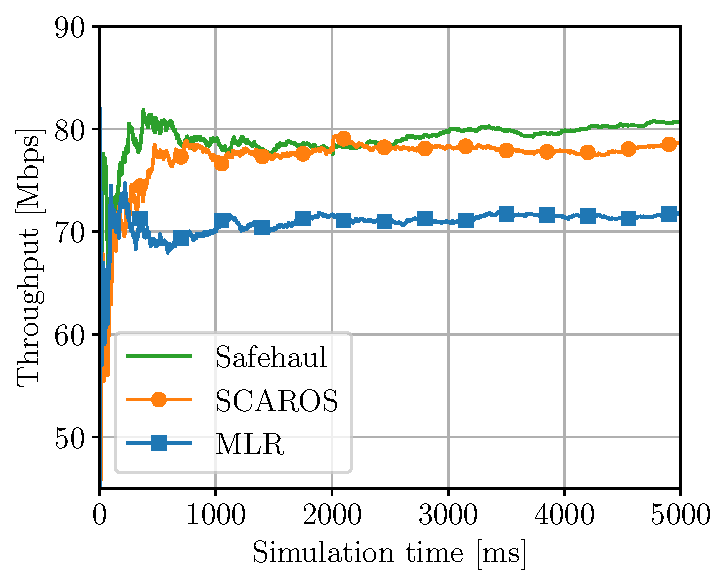
\includegraphics[width=.45\linewidth]{Figures/Safehaul/S1_thr_vs_time.pdf}
    \label{fig:avgTput}
    }
\hfill
\subfloat[][Average per-UE packet drop rate]{
    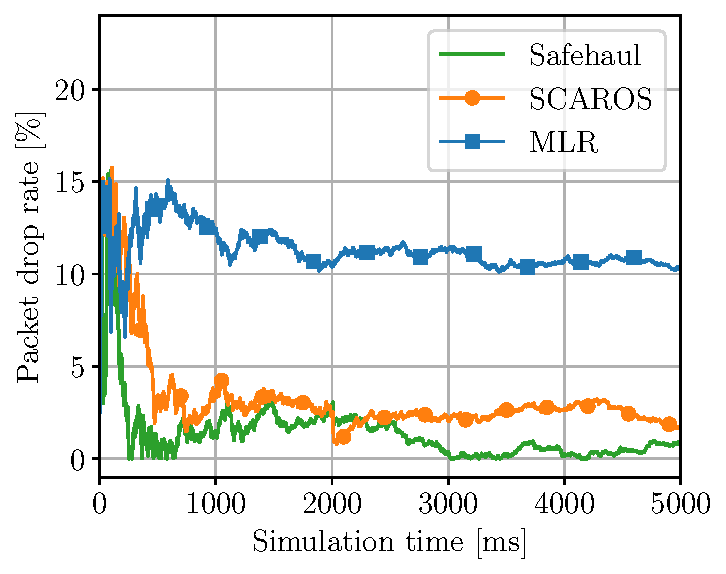
\includegraphics[width=.45\linewidth]{Figures/Safehaul/S1_drop_vs_time.pdf}
    \label{fig:avgDropRate}
    }
  
\caption{Average network performance for $50$ \glspl{ue} and $80$~Mbps per-UE source rate (Scenario 1).}
  \label{fig:avgNetPerfomance}
\end{figure*}
\begin{figure*}[t!]
\centering
\subfloat[][Per-UE end-to-end Latency]{
    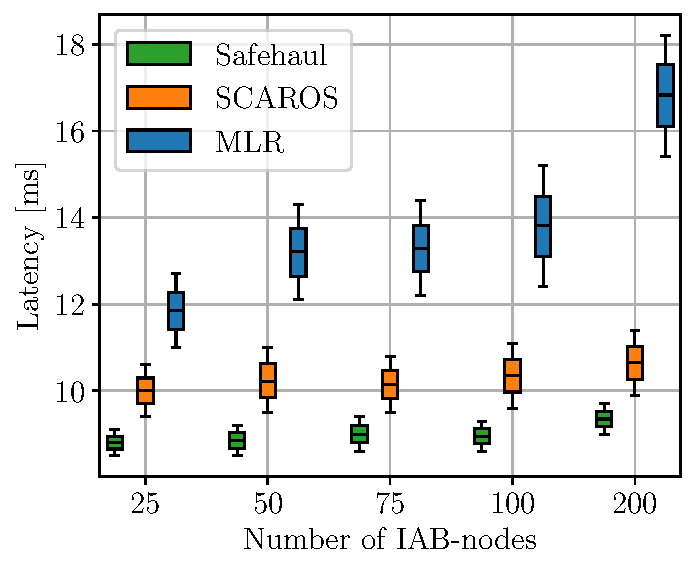
\includegraphics[width=.45\linewidth]{Figures/Safehaul/S2_lat.pdf}
    \label{fig:avgE2EDelay_s2}
    }
\subfloat[][Per-UE throughput]{
    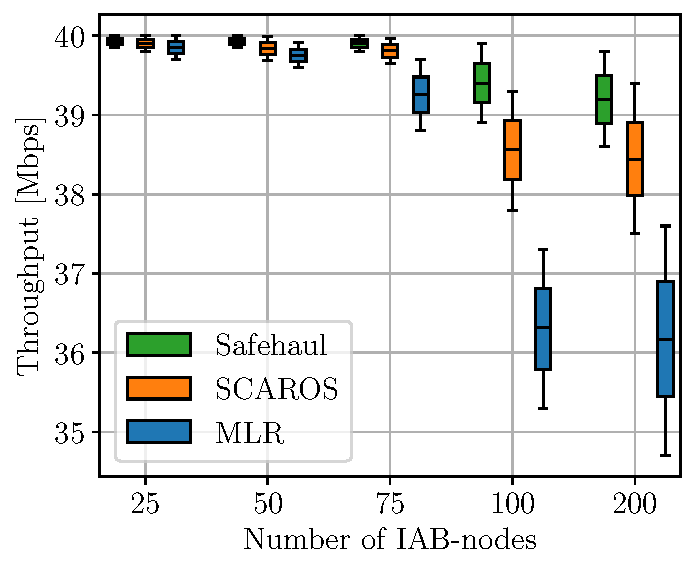
\includegraphics[width=.45\linewidth]{Figures/Safehaul/S2_thr.pdf}
    \label{fig:avgTput_s2}
    }
\hfill
\subfloat[][Per-UE packet drop rate]{
    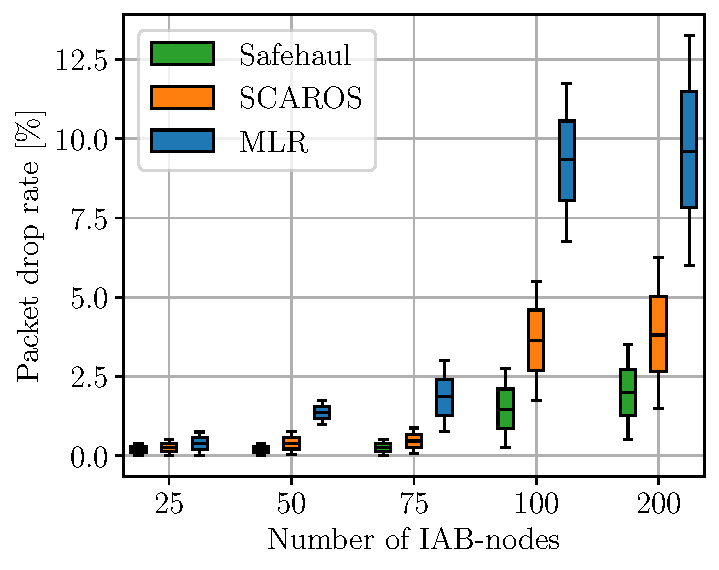
\includegraphics[width=.45\linewidth]{Figures/Safehaul/S2_drop.pdf}
    \label{fig:avgDropRate_s2}
    }
   \caption{Network performance for $\{25, 50, 75, 100, 200\}$ \node{}, $2$ UEs per \nodes{} on average, and $40$ Mbps per-UE source rate (Scenario 2).}
  \label{fig:avgNetPerfomance_s2}
  \vspace*{-3mm}
\end{figure*}

In our simulations, we consider realistic cellular base station deployments in Manhattan, New York City\footnote{The locations correspond to the network of T-Mobile, which has the largest deployment among the \glspl{mno}.} and in the historical city center of Padova. Specifically, for the former we collect the locations of $N=223$ 5G-NR base stations in an area of 15~$\text{Km}^2$ as depicted in Figure~\ref{fig:manhattan}. On the other hand, in the Padova topology we combine locations of $N=100$ 4G-LTE \gls{bs} of different \glspl{mno} (WINDTRE, TIM, and Vodafone) in an area of 10~$\text{Km}^2$ as depicted in Figure~\ref{fig:Padova_Map}, due to the lack of 5G-NR base station deployment at the time of writing of this thesis. The detailed simulation parameters are provided in Table \ref{Tab:parameters-safehaul}. We used the channel model outlined by 3GPP in TR 38.901 \cite{3gpp.38.901}, which provides a statistical channel model for 0.5-100 GHz, and analyzed the "Urban Micro (UMi)-StreetCanyon" scenario.

\begin{table}[t]
\caption{Simulation parameters.}
\centering
\resizebox{0.8\columnwidth}{!}{\label{Tab:parameters-safehaul}
\centering
\scriptsize
\begin{tabular}{l|l}
    \toprule
    Parameter & Value \\ \midrule
    Carrier frequency and bandwidth & 28~GHz and 400~MHz \\
IAB RF chains &   2 (1 access + 1 backhaul) \\
Pathloss model & UMi-Street Canyon \cite{3gpp.38.901} \\
Number of \nodes{} $N$ & \{$223$ NY, $100$ Padova\}   \\
    Source rate & \{40, 80\} Mbps \\
IAB Backhaul and access antenna array & 8H×8V and 4H×4V\\
UE antenna array & 4H×4V\\
IAB and UE height & 15~m and 1.5~m \\
IAB antenna gain & 33~dB \\
    Noise Figure & 10~dB \\
    Risk level $\alpha$ & 0.1\\
    Reliability weight factor $\eta$ & 1\\
\bottomrule
\end{tabular}
}\end{table}

\textbf{Benchmarks.} To provide better insights on the performance of \name{}, we replicate two approaches from the state of the art: $(i)$ \gls{scaros}, a learning-based approach that minimizes the average latency in the network~\cite{ortiz2019scaros}, and $(ii)$ \gls{mlr}, a greedy approach aiming to maximize throughput by selecting the links with the highest data rate.


Our evaluation consists of six scenarios, in which we study the convergence of the algorithms to a steady state, the number of \nodes{}, the number of \donors{}, and the impact of risk aversion. When demonstrating the results, we show the average throughput, latency, and packet drop rate per UE. Furthermore, we show the statistical variance of the obtained results using candlesticks which include the corresponding max, min, mean, and 10 and 90 percentiles. 

\subsubsection{Scenario 1: Average Network Performance}
\label{sub:netPerformance}
Analyzing the performance of the algorithms as a function of time is crucial to determine the convergence speed of the learning-based techniques, i.e.,  \name{} and \gls{scaros}. Hence, in Figure~\ref{fig:avgNetPerfomance} we show the average network performance over time for three metrics: latency, throughput, and packet drop rate.

In Figure~\ref{fig:avgE2EDelay}, we can observe that \name{} rapidly converges to an average latency of approximately $8.6$ ms which is $12.2$\% and $43.4$\% lower than the latency of \gls{scaros} and \gls{mlr}, respectively. The high performance of \name{} stems from the joint minimization of the average latency and the expected value of its tail loss, which results in avoiding risky situations where latency goes beyond $T_\mathrm{max}$.
This is not the case for \gls{scaros} where we observe a high peak in the latency before convergence, i.e., between zero and 1000~ms. \textit{It is exactly the avoidance of such transients in \name{} that leads to higher reliability in the system.} The reliability offered by \name{} allows \glspl{mno} to deploy self-backhauling in an online fashion and without disrupting the network operation. The performance of \gls{mlr} is constant throughout the simulation, as it is not designed as an adaptive algorithm.


Figure \ref{fig:avgTput} shows that the risk-aversion capabilities of \name{} have no negative impact on the average throughput of the network. 
The performance of \name{} is comparable to that of \gls{scaros}, approximately $79.3$ Mbps, and $11.7$\% larger than the performance of \gls{mlr}.
The performance shown in Figure \ref{fig:avgDropRate} is consistent with the behavior observed in Figure \ref{fig:avgE2EDelay}. As \name{} additionally minimizes the $\alpha$-worst latency, it achieves the lowest packet drop rate compared to the reference schemes, namely, $30.1$\% ($84.0$\%) lower than \gls{scaros} (\gls{mlr}).


\subsubsection{Scenario 2: Impact of the Network Size}
\label{sub:netSize}
In Figure~\ref{fig:avgNetPerfomance_s2} we evaluate the reliability of the three considered approaches for different network sizes. Specifically, we vary the number of \nodes{} from 25 to 200.  At the same time, we increase the load in the network by increasing the number of \gls{ue}s.
From the figures, we can clearly see that \name{} consistently achieves a lower variation compared to the reference schemes. This verifies that \name{} achieves the intended optimization goal, i.e., the joint minimization of the average end-to-end delay and its expected tail loss.

Figure~\ref{fig:avgE2EDelay_s2} shows that \name{} is able to maintain an almost constant latency as the number of \nodes{} increases. Specifically, the variation of latency with \name{} is  56.1\% and 71.4\% less than with \gls{scaros} and \gls{mlr}, respectively. Furthermore, \name{} achieves 11.1\% and 43.2\% lower latency compared to \gls{scaros} and \gls{mlr}, where the high variance exhibited by the latter is due to a lack of adaptation capabilities. 

As shown in Figure~\ref{fig:avgTput_s2}, the average throughput of the learning-based approaches \name{} and \gls{scaros} remains constant for the different values of the network size. However, the lowest variation in the  throughput is achieved by \name{}, i.e., only $0.90$ compared to $1.9$ and $2.8$ in the benchmark schemes. Such behavior corroborates \name{}'s reliability capabilities. 

The packet drop rate for different numbers of \nodes{} is shown in Figure~\ref{fig:avgDropRate_s2}. \name{} not only consistently outperforms the reference schemes, but also has the minimum variation in the results (at least $47.3$\% lower compared to the benchmarks). Considering the largest network size and load, i.e., 200 \nodes{} and 400 \glspl{ue}, \name{} achieves $49.3$\% and $81.2$\% lower packet drop rate compared to \gls{scaros} and \gls{mlr}, respectively. 

\subsubsection{Scenario 3: Impact of the number of \donors{}}
\label{sec:multiDonors}
Although the benchmark schemes do not support multiple \donors{}, \name{} is designed to accommodate such scenarios. In Figure~\ref{fig:avgNetPerfomance_s3}, we investigate the impact of the number of \nodes{} on \name{}. To this end, we keep the number of \glspl{ue} and their data rate constant. 
\begin{figure*}[t!]
\centering
\subfloat[][Average per-UE end-to-end Latency]{
    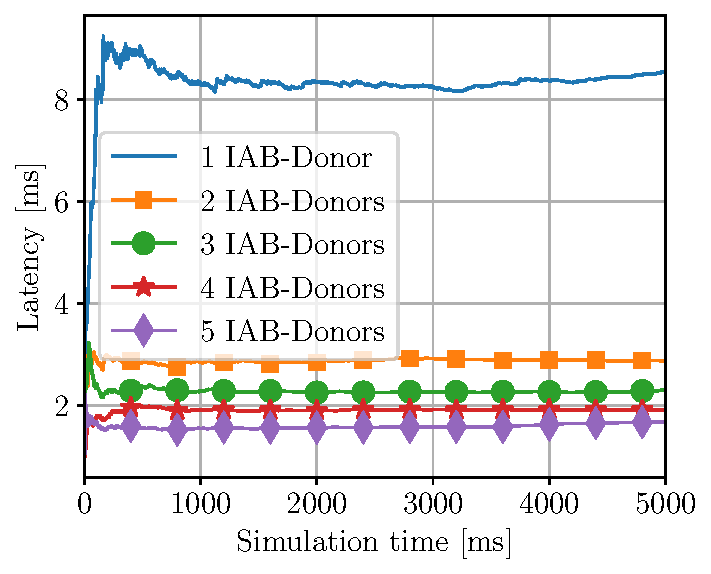
\includegraphics[width=.45\linewidth]{Figures/Safehaul/S3_lat.pdf}
    \label{fig:avgE2EDelay_s3}
    }
\subfloat[][Average per-UE throughput]{
    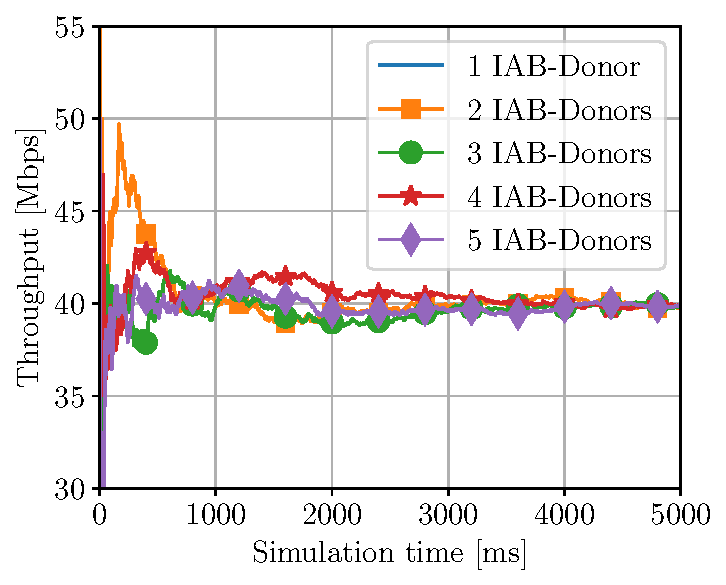
\includegraphics[width=.45\linewidth]{Figures/Safehaul/S3_thr.pdf}
    \label{fig:avgTput_s3}
    }
\hfill
\subfloat[][Average per-UE packet drop rate]{
    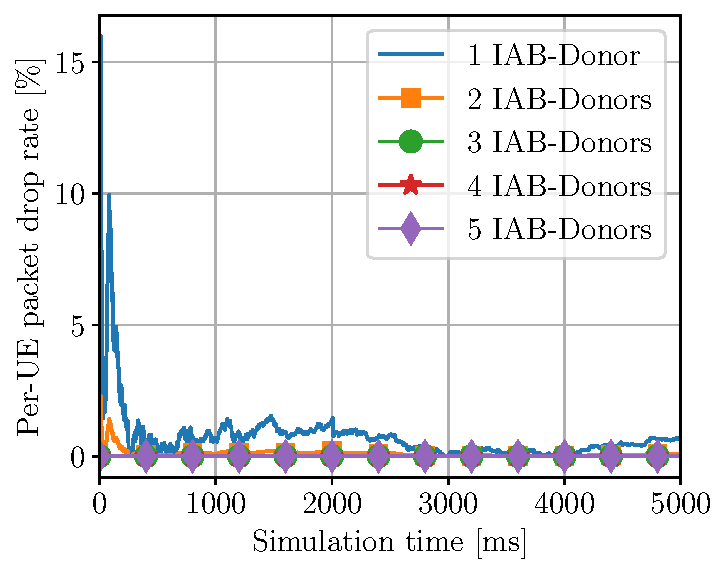
\includegraphics[width=.45\linewidth]{Figures/Safehaul/S3_drop.pdf}
    \label{fig:avgDropRate_s3}
    }
   \caption{Network performance for $50$ \glspl{ue} and $40$ Mbps per-UE source rate, versus the number of \donors{} (Scenario 3).}
  \label{fig:avgNetPerfomance_s3}
  \vspace*{-3mm}
\end{figure*}
We observe in Figure~\ref{fig:avgE2EDelay_s3} that the highest latency is experienced when only one \donor{} is present in the network. This stems from the tributary effect of self-backhauling where the traffic flows towards a central entity which itself can become a bottleneck. As the number of \donors{} increases, the traffic is more evenly distributed, resulting in lower latency. Specifically, the average latency decreases from 8.2~ms for $D=1$ to 1.7~ms when $D=5$. As mentioned, since the load is constant in this scenario, the average throughput also remains constant for all different numbers of \donors{}, see Figure~\ref{fig:avgTput_s3}. Notably, \name{}'s  learning speed is maintained for the different values of $D$.
This is an important design feature of \name{} because having more \donors{} means that the number of paths a \node{} has to the core network increases exponentially. From a learning perspective, such increment implies a larger action set and a lower learning speed. \name{} avoids this problem by learning the average latency based on the estimates of its neighbors and not on the complete paths to the \donors{}.
Finally, Figure \ref{fig:avgDropRate_s3} shows that increasing the number of \donors~significantly reduces the packet drops, which also stems from a better distribution of traffic flows in the network, as observed in Figure~\ref{fig:avgE2EDelay_s3}. 

\begin{figure}[ t!]
    \centering
    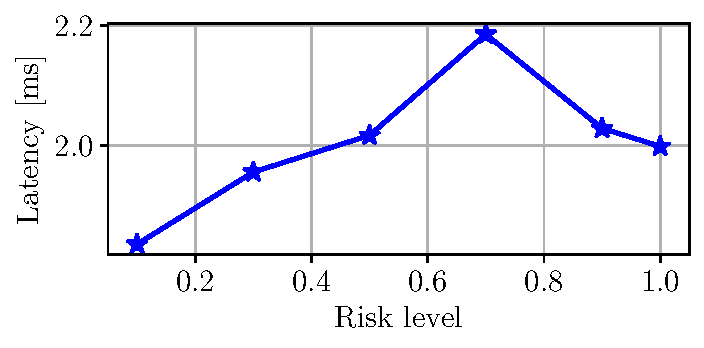
\includegraphics[width=0.6\columnwidth]{Figures/Safehaul/R_latency4.pdf}
    \setlength{\belowcaptionskip}{-12pt}
      \caption{Average latency for 50 UEs and 20 Mbps per-UE source rate, versus the risk level $\alpha$ (Scenario 4)}
      \label{fig:riskParam}
\end{figure}

\subsubsection{Scenario 4: Impact of the risk parameter $\alpha$}
The definition of losses in the tail of the latency distribution is controlled by the risk level parameter $\alpha$. Its impact on the average latency is shown in Figure \ref{fig:riskParam}, where an increasing behavior is observed for $\alpha\leq 0.7$. The lowest latency is achieved for $\alpha=0.1$, which corresponds to the most risk-averse, and therefore the most reliable, case out of all the considered ones.
The non-monotonic behavior of the average latency versus $\alpha$ can be explained by the so-called exploration-exploitation trade-off: the higher $\alpha$, the higher the level of risk, which in turn leads \name{} to learn more about the environment and choose a more reliable action. Eventually, as $\alpha$ grows beyond approximately $0.7$, the performance of \name{} tends to that of the risk-neutral case. As a consequence, the algorithm undertakes excessive exploration, which causes a degradation of the average latency performance.


\begin{figure*}[t!]
\centering
\subfloat[][Average per-UE end-to-end latency]{
    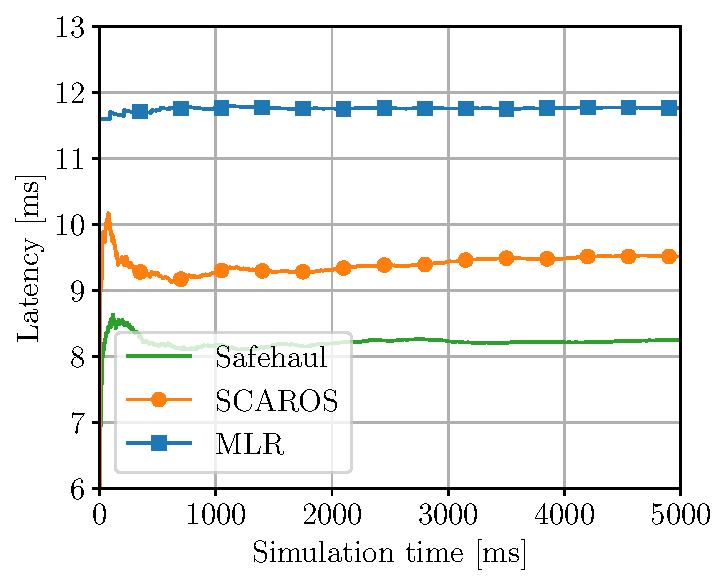
\includegraphics[width=.45\linewidth]{Figures/Safehaul/S1_lat_vs_time_padova.pdf}
    \label{fig:avgE2EDelayPadova}
    }
\subfloat[][Average per-UE throughput]{
    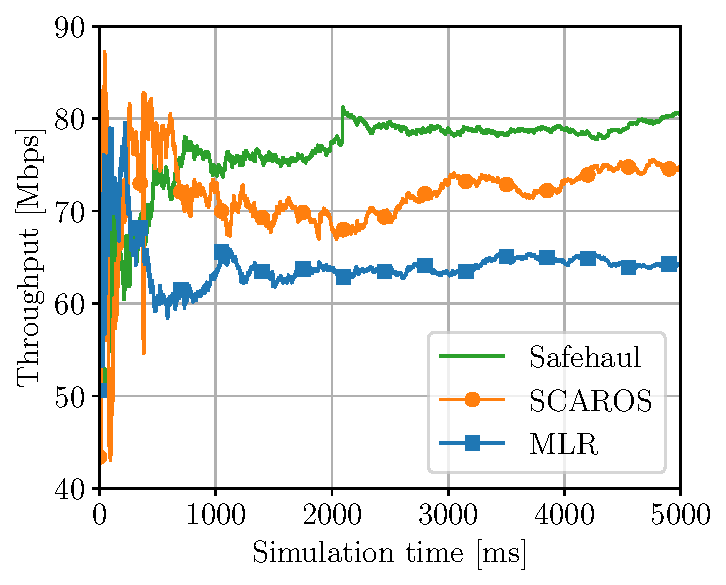
\includegraphics[width=.45\linewidth]{Figures/Safehaul/S1_thr_vs_time_padova.pdf}
    \label{fig:avgTputPadova}
    }
\hfill
\subfloat[][Average per-UE packet drop rate]{
    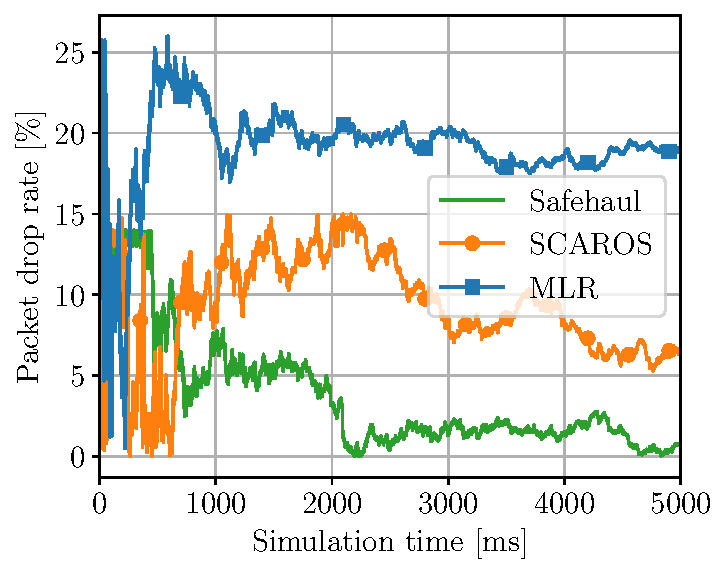
\includegraphics[width=.45\linewidth]{Figures/Safehaul/S1_drop_vs_time_padova.pdf}
    \label{fig:avgDropRatePadova}
    }
  
\caption{Average network performance for $50$ \glspl{ue} and $80$~Mbps per-UE source rate (Scenario 1) in Padova.}
  \label{fig:avgNetPerfomancePadova}
\end{figure*}


\begin{figure*}[t!]
\centering
\subfloat[][Per-UE end-to-end Latency]{
    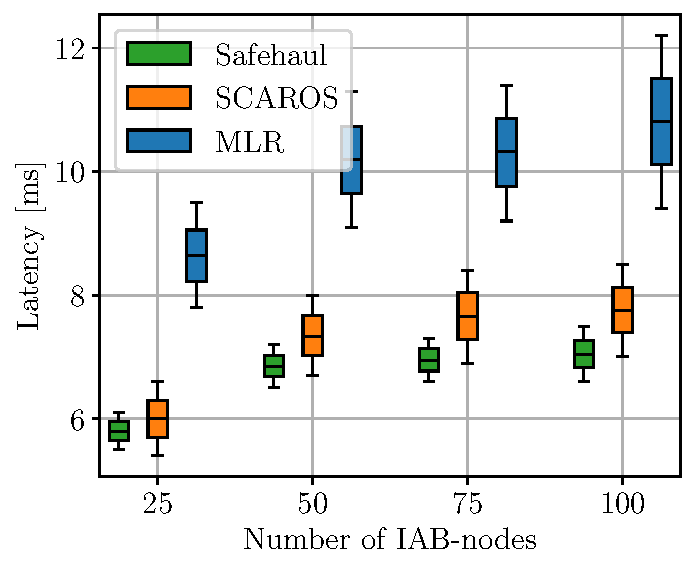
\includegraphics[width=.45\linewidth]{Figures/Safehaul/S2_lat_padova.pdf}
    \label{fig:avgE2EDelay_s2Padova}
    }
\subfloat[][Per-UE throughput]{
    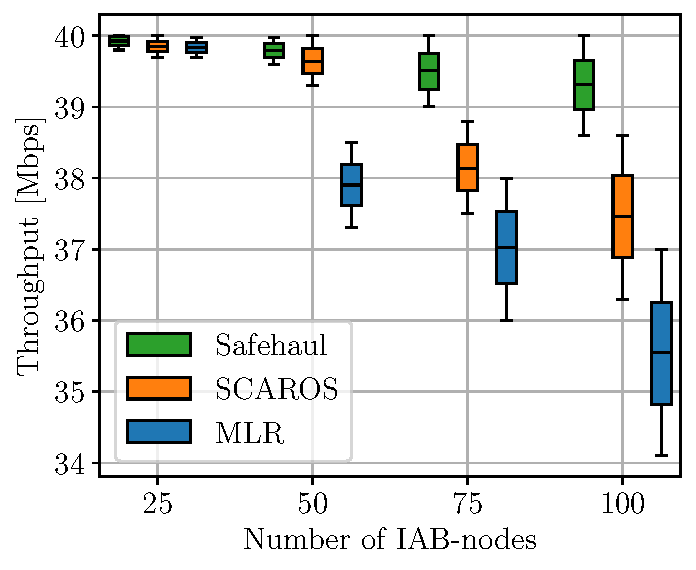
\includegraphics[width=.45\linewidth]{Figures/Safehaul/S2_thr_padova.pdf}
    \label{fig:avgTput_s2Padova}
    }
\hfill
\subfloat[][Per-UE packet drop rate]{
    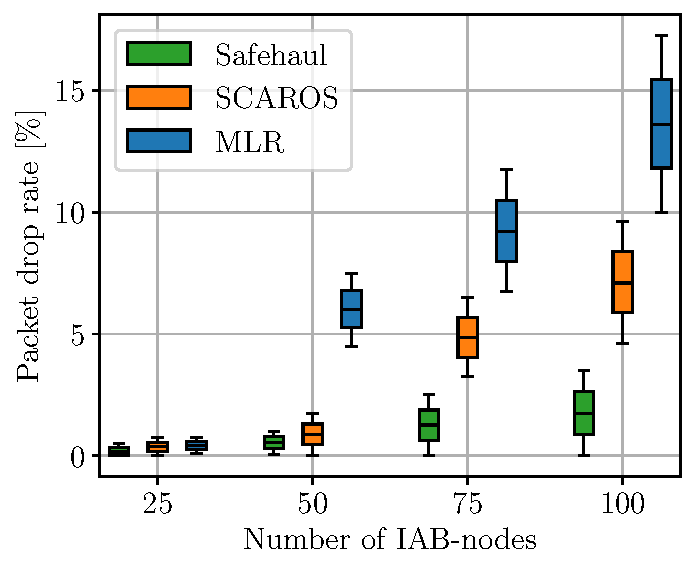
\includegraphics[width=.45\linewidth]{Figures/Safehaul/S2_drop_padova.pdf}
    \label{fig:avgDropRate_s2Padova}
    }
   \caption{Network performance for $\{25, 50, 75, 100\}$ \nodes{},$2$ UEs per \node{} on average, and $40$ Mbps per-UE source rate (Scenario 2) in Padova.}
  \label{fig:avgNetPerfomance_s2Padova}
  \vspace*{-3mm}
\end{figure*}

\begin{figure*}[t!]
\centering
\subfloat[][Average per-UE end-to-end Latency]{
    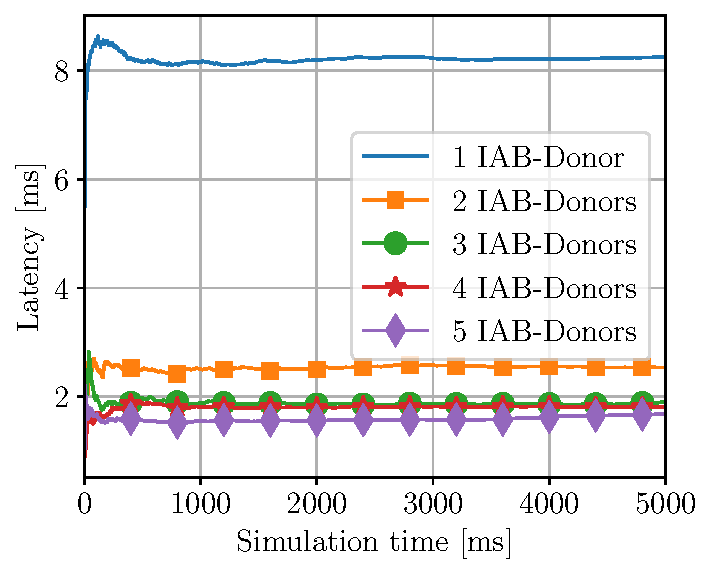
\includegraphics[width=.45\linewidth]{Figures/Safehaul/S3_lat_padova.pdf}
    \label{fig:avgE2EDelay_s3Padova}
    }
\subfloat[][Average per-UE throughput]{
    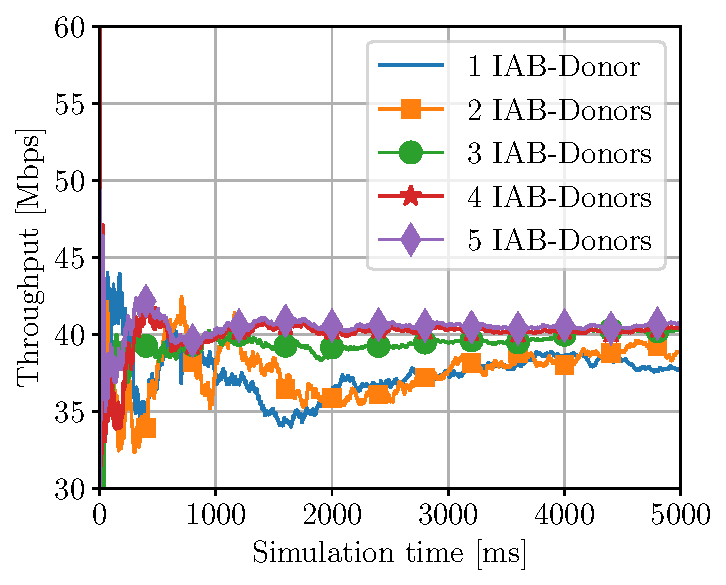
\includegraphics[width=.45\linewidth]{Figures/Safehaul/S3_thr_padova.pdf}
    \label{fig:avgTput_s3Padova}
    }
\hfill
\subfloat[][Average per-UE packet drop rate]{
    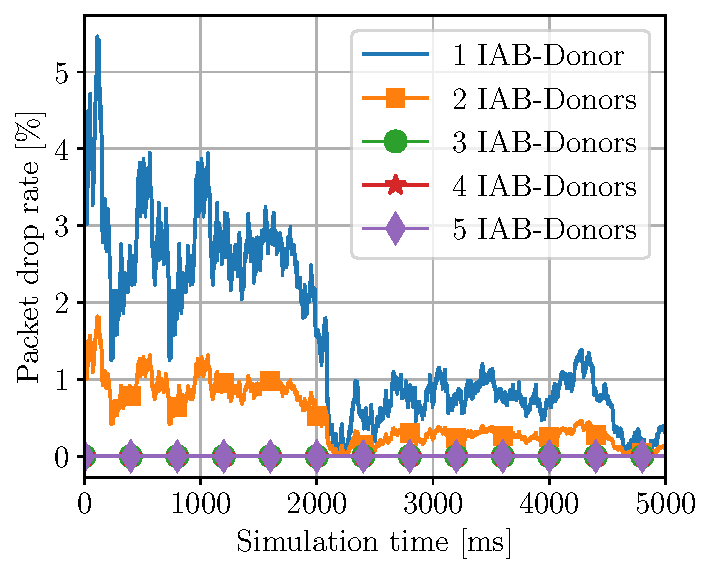
\includegraphics[width=.45\linewidth]{Figures/Safehaul/S3_drop_padova.pdf}
    \label{fig:avgDropRate_s3Padova}
    }
  
   \caption{Network performance for $50$ \glspl{ue} and $40$ Mbps per-UE source rate, versus the number of \donors{} in Padova (Scenario 3).}
  \label{fig:avgNetPerfomance_s3Padova}
  \vspace*{-3mm}
\end{figure*}

\subsubsection{Scenario 5: Performance in different topologies}


To verify the generality of the proposed algorithms, it is essential to examine how they perform in different topologies, and consider both typical network performance metrics (i.e., along the lines of Scenario 1) and their stability with respect to the number of \nodes{} and \donors{} (Scenarios 2 and 3). To this end, we ran additional simulations in the deployment depicted in Figure~\ref{fig:Padova_Map}, which mimics the \nodes{} locations of the historic center of Padova. We report the average network performance over time, in terms of end-to-end packet drop rate, throughput, and latency in Figure~\ref{fig:avgNetPerfomancePadova}. Overall, the outcomes of this simulation campaign are in line with those obtained in Scenario 1. 
Specifically, as seen in Figure~\ref{fig:avgE2EDelayPadova}, \name{} quickly converges to an average latency of approximately 8~ms, which is 14\% and 31\% lower than SCAROS and MLR's latency. Figure~\ref{fig:avgTputPadova} shows the average per-UE throughput, for which \name{} achieves about 4\% and 17\% better performance than SCAROS and MLR, respectively. Similarly, the performance depicted in Figure~\ref{fig:avgDropRatePadova} is in line with that reported  in Figs.~\ref{fig:avgE2EDelayPadova} and ~\ref{fig:avgTputPadova}, with \name{} achieving approximately a 24\% and 38\% smaller packet drop rate than SCAROS and MLR, respectively. 

In Figure~\ref{fig:avgNetPerfomance_s2Padova}, we compare the consistency of the performance of the three algorithms with respect to the network size. In particular, we change the number of \nodes{} from 25 to 100, keeping fixed the number of UEs per \node{} and thus effectively increasing the network load on the \donor{}. 
Results show that \name{}, when compared to other schemes, exhibits minimal performance degradation when introducing additional \nodes{} and \glspl{ue}. As can be seen in Figure~\ref{fig:avgE2EDelay_s2Padova}, the latency achieved by \name{} increases by at most 16\% in the case of 100 \nodes{}, while SCAROS and MLR lead to a latency which is consistently higher and increases up to~27\% and ~25\% when deploying additional nodes, respectively.
Similar trends can be observed in Figs.~\ref{fig:avgTput_s2Padova} and \ref{fig:avgDropRate_s2Padova}, which report throughput and packet loss versus the network size, respectively. Indeed, \name{} is the best performer across the whole range of \nodes{} which have been considered. Furthermore, \name{} loses 20\% more packets with the denser network deployment (i.e., 100 \nodes{}), while reference schemes exhibit an increase in packet loss of up to 33\%. 

We complete this analysis by examining how the number of donors affects the performance achieved by \name{} in the Padova-like topology. 
As can be seen in Figure~\ref{fig:avgNetPerfomance_s3Padova}, increasing the number of fiber-backhauled base stations progressively reduces the latency. Similarly, and in line with the results obtained in Scenario 3 and reported in Figure~\ref{fig:avgDropRate_s3Padova}, the packet drop rate varies from approximately 0.08\% when considering a single \donor{}, to approximately 0.003\% in the presence of five \donors{}. The performance improvements introduced by additional fiber links saturate after 3 donors, thanks to the efficient routing and scheduling performed by \name{}.

In summary, the results obtained in the additional topology mimicking the historical center of Padova are well aligned with those obtained in the Manhattan topology. Although the specific values of the network metrics achieved by the considered schemes in the two topologies are different (for instance, SCAROS achieves a 66\% lower packet drop rate in Scenario~1 compared to Scenario~5), the trends among the various schemes are the same. Specifically, we observed that \name{} consistently achieves the best performance in comparison to SCAROS and MLR across different metrics, which supports the claim that the proposed scheduler is capable of learning how to optimize arbitrary deployment topologies.

\subsubsection{Scenario 6: Network resilience}
In networking, resilience refers to the ability of a network to recover in a quick and effective fashion from disruptions, thus providing reliable and high-quality communication services to its users.
Specifically, the ability to recover from link failures is particularly important in \gls{iab} networks, where backhaul links are susceptible to the typical disruptions which plague the \gls{ran} due to its mobile and wireless nature. For instance, the links among \nodes{} can be degraded by adverse environmental conditions such as heavy rain and monsoons, physical obstacles and network congestion. These disruptions can cause temporary or permanent communication failures, which in turn result in degraded performance and/or loss of connectivity for the end users. 
To prevent and/or recover from these undesired events, a backhaul scheduler must detect, mitigate, and recover from various types of disruptions and failures, and must maintain the required level of service availability and performance despite the time-varying channel conditions.

\begin{figure*}[t!]
\centering
\subfloat[][Average per-UE end-to-end latency]{
    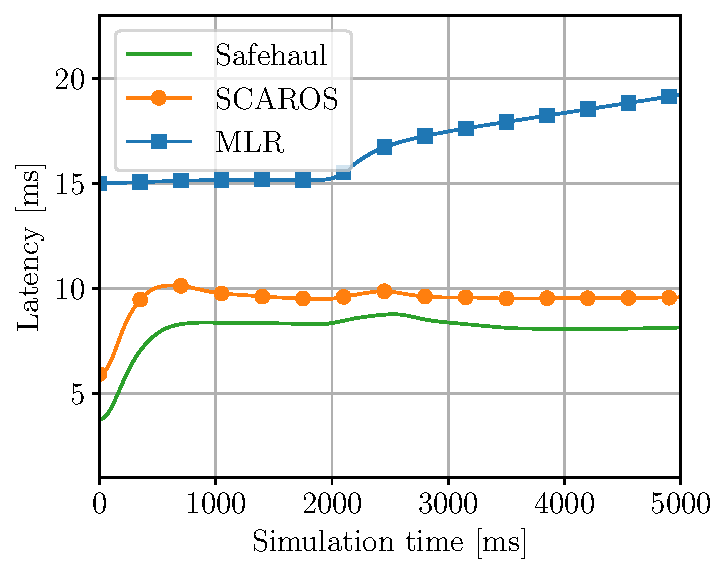
\includegraphics[width=.45\linewidth]{Figures/Safehaul/S6_lat_vs_time.pdf}
    \label{fig:avgE2EDelay_Re}
    }
\subfloat[][Average per-UE throughput]{
    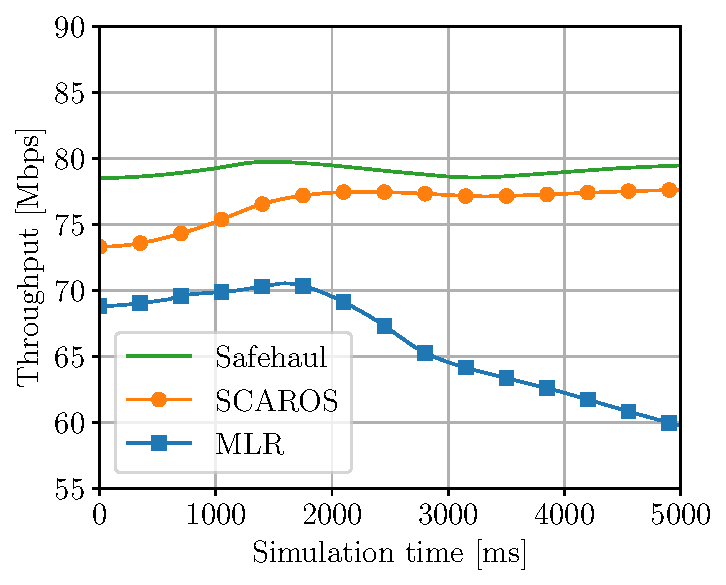
\includegraphics[width=.45\linewidth]{Figures/Safehaul/S6_thr_vs_time.pdf}
    \label{fig:avgTput_Re}
    }
\hfill
\subfloat[][Average per-UE packet drop rate]{
    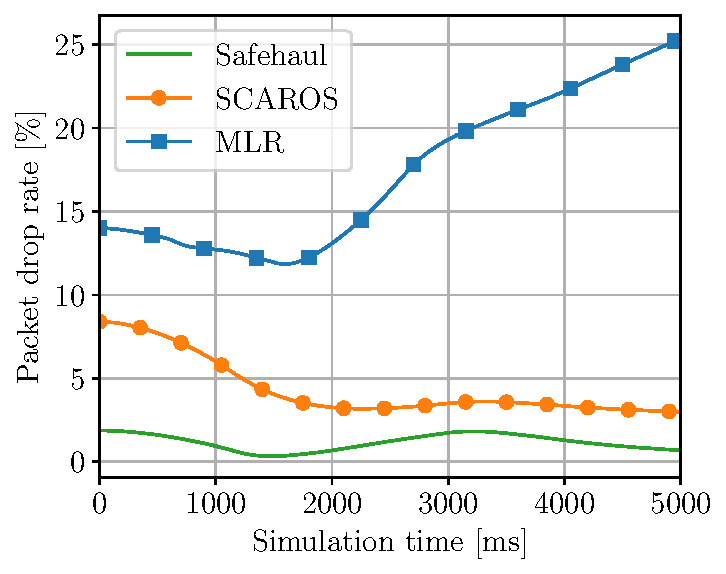
\includegraphics[width=.45\linewidth]{Figures/Safehaul/S6_drop_vs_time.pdf}
    \label{fig:avgDropRate_Re}
    }
  
\caption{Average network performance for $50$ \glspl{ue} and $80$~Mbps per-UE source rate where 1 random \node{} is shut down.}
  \label{fig:avgNetPerfomance_Re}
\end{figure*}


\begin{figure*}[t!]
\centering
\subfloat[][Average per-UE end-to-end latency]{
    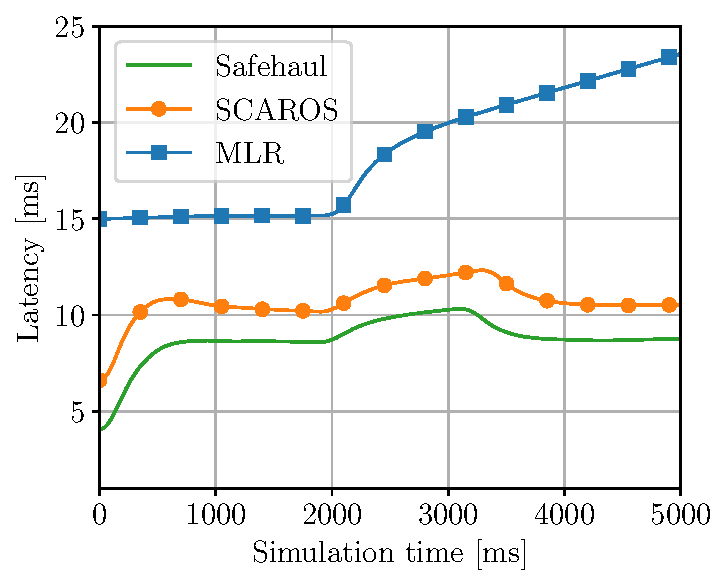
\includegraphics[width=.45\linewidth]{Figures/Safehaul/S7_lat_vs_time.pdf}
    \label{fig:avgE2EDelay_Re2}
    }
\subfloat[][Average per-UE throughput]{
    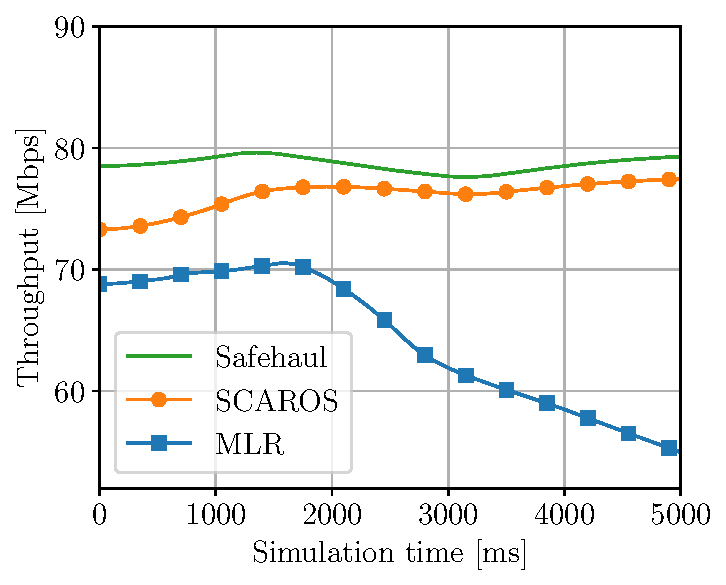
\includegraphics[width=.45\linewidth]{Figures/Safehaul/S7_thr_vs_time.pdf}
    \label{fig:avgTput_Re2}
    }
\hfill
\subfloat[][Average per-UE packet drop rate]{
    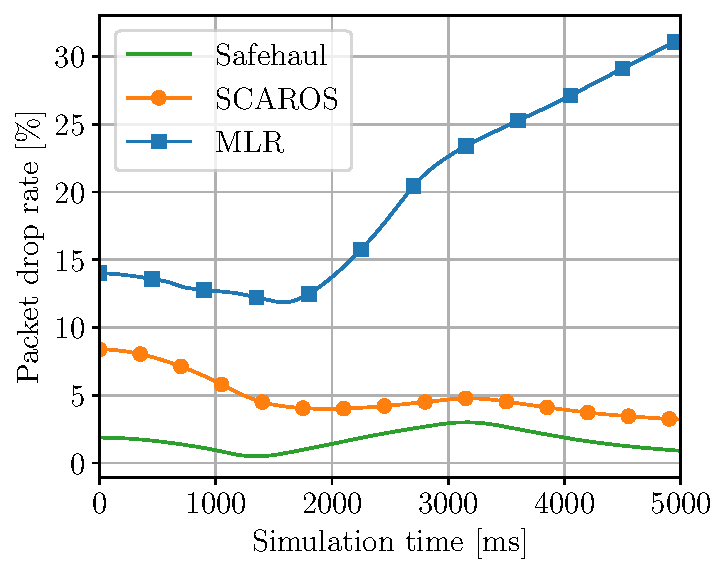
\includegraphics[width=.45\linewidth]{Figures/Safehaul/S7_drop_vs_time.pdf}
    \label{fig:avgDropRate_Re2}
    }
  
\caption{Average network performance for $50$ \glspl{ue} and $80$~Mbps per-UE source rate where 3 random \nodes{} are shut down.}
  \label{fig:avgNetPerfomance_Re2}
\end{figure*}

We benchmark the resilience of the proposed algorithm by mimicking radio link failures, which we simulate by stopping \nodes{} at a fixed time instant (2000~s), and inspecting the resulting performance degradation.
Since the failed node(s) is (are) chosen at random, we run multiple simulations to estimate the average network performance, as shown in Figs.~\ref{fig:avgNetPerfomance_Re} and~\ref{fig:avgNetPerfomance_Re2} for the case of one and three link failures, respectively.

Results show that MLR is unable to react to the link failure(s) due to its static and myopic policy. Specifically, the disruption causes an increase of~33\% (60\%) in latency, and a decrease of up to 15\% (23\%) in throughput when considering one (three) link failure(s).
On the other hand, both \name{} and SCAROS are capable of adapting the scheduling to the new topology. Indeed, both schemes show a transient region where the performance is slightly degraded since the algorithms are learning new routes and resource partitions to account for the lost link. Nevertheless, \name{} and SCAROS eventually converge to a solution which provides approximately the same network performance as before the failures, in both cases of one and three lost links.

\subsection {Related work}
\label{s:related}

Self-backhauling wireless networks have been studied in different contexts. Ranging from the so-called \glspl{hetnet} and \gls{iab} 5G \gls{nr} systems, to \glspl{cran}, each has considered a different set of premises and optimization goals. In this section, we review the related work in the context of basic assumptions and their optimization goals. 

\textbf{Ideal backhaul links.} Numerous works assume either an \textit{infinite or fixed capacity backhaul link}. This is often motivated by the presence of a wired fiber link between the \glspl{sbs} and the \gls{mbs}~\cite{pan2017joint, huang2015joint, nguyen2020nonsmooth, rasekh2015interference}. Indeed, most of these works consider a scenario where a centralized \gls{bbu} is connected to several \glspl{rrh}, i.e., radios which lack signal processing capabilities~\cite{pan2017joint, huang2015joint, nguyen2020nonsmooth}. In particular, the authors of~\cite{nguyen2020nonsmooth} consider an even more complex C-RAN scenario where RRHs feature caching and signal processing capabilities. However, in an \gls{iab} context it is fundamental to consider \textit{limited-rate, time-varying backhaul channels} and to study the impact of such limitations on the performance of the \gls{ran}.

\textbf{Constrained topologies.} It is often assumed that self-backhauled networks have a \textit{specific topology}. This assumption usually simplifies the problem and makes it tractable and/or solvable in polynomial time. For instance, the authors of~\cite{kwon2019joint, pizzo2017optimal, lei2020deep} assume a single-hop network where each \gls{sbs} is directly connected to the \gls{mbs}. In~\cite{kulkarni2018max}, a $k$-ring deployment is considered, i.e., a topology where a single \gls{iab}-donor provides backhaul connectivity to $k$ rings of \gls{iab}-nodes. Even though this topology can be used to model networks with arbitrary depth, it maintains a symmetric load for each node, an assumption which generally does not hold in real networks.
In fact, the 3GPP does not impose any limits on the number of \gls{iab}-nodes which can be connected to a given \gls{iab}-donor, nor does it set an upper bound on the number of wireless hops from the latter to other wireless-backhauled base stations~\cite{3gpp_38_874}. Accordingly, in our problem formulation we consider \gls{iab} networks with an \textit{arbitrary number of nodes and an arbitrary maximum number of wireless hops} between \glspl{mbs} and \glspl{sbs}. 

\textbf{Simplistic traffic models.} Some works either assume a \textit{full buffer traffic model and/or impose flow conservation constraints}. In particular, the authors of~\cite{yuan2018optimal, rasekh2015interference} consider systems where the capacity of each link can  always be fully exploited thanks to the presence of \textit{infinite data to transmit at each node}. However, in actual \gls{iab} deployments the presence of packets at the \glspl{mbs} and \glspl{sbs} is conditioned on the \textit{status of their \gls{rlc} buffers and, in turn, on the previous scheduling decisions}. Moreover, \textit{packets can actually be buffered at the intermediate nodes}, thus preventing the need for transmitting a given packet in consecutive time instants along the whole route from the \gls{iab}-donor to the \glspl{ue} (or vice versa). 

\textbf{Optimization goals.} The works in the literature focus on different optimization goals. Therefore, they prioritize different network metrics. For instance, the authors of~\cite{hur2013millimeter} aim to optimize the beam alignment between \glspl{mbs} and \glspl{sbs}. Instead, the work of~\cite{alizadeh2019load} aims to compute the optimal user-to-base-station association. However, they neglect backhaul associations and focus on the access only. In~\cite{kwon2019joint, alizadeh2019load, zhu2016qos, yuan2018optimal} the objective function is a function of the users data-rate. In particular, the authors of~\cite{yuan2018optimal} optimize the max-min user throughput, arguing that such a metric better captures the performance of the bottleneck links. In~\cite{vu2018path}, the average rate of each link is maximized under bounded delay constraints. In our work, we focus on reliability by minimizing not only the average end-to-end delay, but also the expected value of the worst-case performance.
The work closest to this article is SCAROS~\cite{ortiz2019scaros},  a learning-based latency-aware scheme for resource allocation and path selection in self-backhauled networks. Assuming a single IAB-donor, the authors study arbitrary multi-tier \gls{iab} networks considering the impact of interference and network dynamics. In contrast, we aim at enhancing the reliability of the IAB-network by jointly minimizing the average end-to-end delay and its expected tail loss. 

\subsection*{Appendix}
\label{sec:appendix}
For the proof of Proposition \ref{prop:probNonOptArm}, Theorem 3 in \cite{Luo2017} is needed. For completeness, we first present the theorem in \cite{Luo2017} for the special case in which the considered random variables are independent. Next, we present the proof of Proposition \ref{prop:probNonOptArm}.
\begin{theorem} \label{eq:Theorem2_part2}
Let $T_{a_n,i}$ be independent random variables where $\max_{1\leq j\leq i}{T_{a_n,j}} = T_\mathrm{max}$, with $i\in\{1,2,...\}$.
Then, for any $0 < \delta \leq 1/2$, $\xi > 0$ and $\gamma > 0$, there exists a positive constant $C$ which only depends on $\xi$ and $\gamma$, such that the probability of the event $|\estcvar{a_n,i}-\cvar{a_n,i}| \geq 2\xi\alpha^{-1}T_{\max} i^{-\delta}(\ln{\ln{i}})^{1/2}\ln{i}$ is smaller than or equal to $Ce^{-(1+\gamma)\ln i}$.
\end{theorem}
\begin{proof}
See Theorem 3 in \cite{Luo2017}.
\end{proof}

\subsection*{Proof of Proposition \ref{prop:probNonOptArm}}
\begin{proof}[\unskip\nopunct]

In this proof, we use the result of the regret bound for the risk-neutral case without CVaR, shown in \cite[Theorem 3]{Auer2002}, as a basis. Additionally, we use the bound for the terms related to the CVaR formulated in \cite[Theorem 3]{Luo2017}. 
Using both these results, we first bound the probability that Safehaul chooses a suboptimal arm in the exploitation phase. Then, we combine the latter with the probability of choosing a suboptimal arm in the exploration phase to derive the bound given in Proposition~\ref{prop:probNonOptArm}.

From the system model and Proposition \ref{prop:probNonOptArm}, we have that $c > 0$, $0 < d \leq 1$, and 
$\epsilon_n := \min(1, \frac{cA_n}{d^2i})$. 
Moreover, $a_{n,i}$ is the action chosen by $\epsilon$-greedy in time slot $i$ and $K_{a_n, i}$ is the number of times, up to time slot $i$, in which \name{} chose action $a_n$ \textit{at random}. Similarly, we use $K^*_{i}$ for the counter of the optimal action.
$T_{a_n, i}$ are independent random variables distributed according to the rewards linked to action $a_n$. We use $T_i^*$ for the optimal action, and $\hat{T}_{a_n, i}$ is the estimated mean of the probability distribution of the rewards linked to action $a_n$ using $K_{a_n,i}$ samples. As before, we use $\hat{T}^*_{i}$ for the optimal action.
$\estcvar{a_n, i}$ is the estimated \gls{cvar} of action $a_n$ up to time slot $i$ and $\estcvar{i}^*$ is the estimated \gls{cvar} of the optimal action up to time slot $i$.
Then, the probability that action $a_n$ is chosen in time slot $i$ is upper bounded as
{\small
 \begin{align}
     \label{eq:inicProbAction}
    \mathbb{P}[a_{n,i} = a_n] \leq & \mathbb{P}\left[\delta_{a_n,i-1} \leq \delta_{i-1}^* \right]\left(1 - \frac{\epsilon_i}{A_n} \right) + \frac{\epsilon_i}{A_n},
\end{align} }
 with $\delta_{a_n,i-1} = \hat{T}_{a_n, i-1} + \eta \estcvar{a_n, i-1}$ and $\delta^*_{i-1} = \hat{T}^*_{i-1} + \eta \estcvar{i-1}^*$.
The first term in \eqref{eq:inicProbAction} is the probability of exploitation and the second term to the probability of exploration. \\ 
Using the mean $\Bar{T}_{a_n}$ and $\cvar{a_n}$ of action $a_n$, and the likewise defined $\Bar{T}^*$ and $\cvar{}^*$ for the optimal action, we set $\Delta^\mathrm{mean}_{a_{n}} := \Bar{T}_{a_n} - \Bar{T}^*$ and $\Delta^\mathrm{cvar}_{a_{n}} := \cvar{a_n} - \cvar{}^*$.
Using these definitions in \eqref{eq:inicProbAction} we conclude
{\small
\begin{align}
    \mathbb{P} &\left[\delta_{a_n,i-1} \leq \delta_{i-1}^*\right] \leq \nonumber \\
    &\mathbb{P}\!\left[\delta_{a_n,i-1} \leq \eta \cvar{a_n}  - \frac{\Delta^\mathrm{mean}_{a_n}}{2} + \right. \left. \bar{T}_{a_n}  - \eta \frac{\Delta^\mathrm{cvar}_{a_n}}{2}\right] +\nonumber \\
    &\mathbb{P}\!\left[\bar{T}^* + \frac{\Delta^\mathrm{mean}_{a_n}}{2} + \eta \cvar{}^* +  \eta \frac{\Delta^\mathrm{cvar}_{a_n}}{2} \leq \delta_{i-1}^*\right] \nonumber \\
     & \mathbb{P}\!\left[\hat{T}_{a_n,i-1} \leq \bar{T}_{a_n} - \frac{\Delta^\mathrm{mean}_{a_n}}{2}\right] + \mathbb{P}\!\left[\bar{T}^* + \frac{\Delta^\mathrm{mean}_{a_n}}{2} \leq \hat{T}^*_{i-1}\right] + \nonumber \\
    &\mathbb{P}\!\left[\estcvar{a_n,i-1} \leq \cvar{a_n} - \frac{\Delta^\mathrm{cvar}_{a_n}}{2}\right]+ \nonumber \\
    & \mathbb{P}\!\left[\cvar{}^* + \frac{\Delta^\mathrm{cvar}_{a_n}}{2} \leq \estcvar{i-1}^*\right]. \label{eq:probBrokenDown}
\end{align}
}
Similar to \cite{Auer2002}, we use the Chernoff-Hoeffding bound for the first two terms in \eqref{eq:probBrokenDown}. For the last two  summands, there remains to find a bound for the difference between the \gls{cvar} and its estimate $\estcvar{}$. 
From Theorem \ref{eq:Theorem2_part2}, we set $\xi := {\Delta^\mathrm{cvar}_{a_n} \alpha}/{4 T_{max}}$, $\delta=0.5$ and by using the limit $\gamma \rightarrow 0$, we obtain
{\small
\begin{equation}
\begin{gathered}
    \mathbb{P}\!\left[|\estcvar{a_n,i}-\cvar{a_n,i}|\geq \frac{\Delta^\mathrm{cvar}_{a_n}}{2}i^{-0.5}(\ln{\ln{i}})^{0.5}\ln{i}\right] \leq \frac{C}{i}.
\end{gathered}
\end{equation}
}
As $\max_i i^{-0.5}(\ln{\ln{i}})^{0.5}\ln{i} < 1$, the condition ${(\Delta^\mathrm{cvar}_{a_n}}/{2})i^{-0.5}(\ln{\ln{i}})^{0.5}\ln{i} \leq \frac{\Delta^\mathrm{cvar}_{a_n}}{2}$
holds for all $i$. Therefore, considering the last two summands in \eqref{eq:probBrokenDown}, we conclude that there exists a positive constant $C$ that satisfies
{\small
\begin{equation}
\mathbb{P}\!\left[|\estcvar{a_n,i}-\cvar{a_n,i}|\geq \frac{\Delta^\mathrm{cvar}_{a_n}}{2}\right] \leq \frac{C}{i}.
\label{eq:partialCVaRBound}
\end{equation}}
The number of times action $a_n$ has been selected up to time slot $i$ is smaller than or equal to $i$, i.e., $K_{a_n,i}\leq i$. Using \eqref{eq:partialCVaRBound} we write the last two summands in \eqref{eq:probBrokenDown} as 
{\small
\begin{align}
    \mathbb{P}\!\left[\estcvar{a_n,i-1} \leq \cvar{a_n} - \frac{\Delta^\mathrm{cvar}_{a_n}}{2} \right] \leq \frac{C}{K_{a_n,i-1}},
\end{align}}
and
{\small
\begin{align}
    \mathbb{P}\!\left[\cvar{}^* + \frac{\Delta^\mathrm{cvar}_{a_n}}{2} \leq \estcvar{i-1}^*\right] \leq \frac{C}{K^*_{i-1}}.
\end{align}}
As in \cite{Auer2002}, we use Bernstein's inequality to get an estimate for $K_{a_n,i-1}$. Defining $x_0 := {1}/{2A_n}\sum_{j=1}^{i-1}\epsilon_j$ for $i-1 \geq \frac{cA_n}{d^2}$ we get $P(K_{a_n,i-1} \leq x_0) \leq e^{-\frac{x_0}{5}}$.
Additionally, from \cite{Auer2002}: 
{\small
\begin{equation}
    x_0 \geq \frac{c}{d^2}\ln\left(\frac{(i-1)d^2e^{0.5}}{cA_n}\right) =: C'(i).
\end{equation}}
The same holds for the optimal action and $K^*_{i-1}$. Using these estimations for $x_0$, we can conclude that for $i-1 \geq {cA_n}/{d^2}$
{\small
\begin{align}
    &\mathbb{P}\!\left[\estcvar{a_n,i-1} \leq \cvar{a_n} - \frac{\Delta^\mathrm{cvar}_{a_n}}{2}\right] \\
    &\leq \sum_{j=1}^{i-1} \mathbb{P}[K_{a_n,i-1}=j] \frac{C}{j} \nonumber \\
    &= \sum_{j=1}^{\lfloor x_0 \rfloor} \mathbb{P}[K_{a_n,i-1}=j] \frac{C}{j} + \sum_{j=\lfloor x_0 \rfloor + 1}^{i-1} \mathbb{P}[K_{a_n,i-1}=j] \frac{C}{j} \nonumber\\
    &\leq C x_0 e^{-\frac{x_0}{5}} + \frac{C}{x_0} \leq C x_0 e^{-\frac{x_0}{5}} + \frac{C}{C'(i)}.
\end{align}
}
The same holds again for the optimal action
{\small
\begin{align}
    \mathbb{P}\!\left[\cvar{}^* + \frac{\Delta^\mathrm{cvar}_{a_n}}{2} \leq \estcvar{i-1}^*\right] &\leq C x_0 e^{-\frac{x_0}{5}} + \frac{C}{C'(i)}.
\end{align}}
Together with the bounds from Theorem 3 in \cite{Auer2002} it follows that for $C \geq 1$:
{\small
\begin{align*}
    \mathbb{P}&\left[a_{n,i} = a_n\right] \\
    &\leq \frac{\epsilon_i}{A_n} + 4 C x_0 e^{-\frac{x_0}{5}} + \frac{4}{\left(\Delta^\mathrm{mean}_{a_n}\right)^2}e^{\frac{-\left(\Delta^\mathrm{mean}_{a_n}\right)^2\lfloor x_0 \rfloor}{2}}  + 2 \frac{C}{C'(n)} \nonumber \\
    &\leq \frac{c}{d^2i} +  2 \frac{Cd^2}{c\ln\left(\frac{(i-1)d^2e^{0.5}}{cA_n}\right)}
    + \frac{4e}{d^2}\left(\frac{c A_n}{(i-1)d^2e^{0.5}}\right)^{\frac{c}{2}} +\\
    & \:\:\quad 4C\frac{c}{d^2}\ln\left(\frac{(i-1)d^2e^{0.5}}{c A_n}\right) \left(\frac{c A_n}{(i-1)d^2e^{0.5}}\right)^{\frac{c}{5d^2}}.
\end{align*}
}
\end{proof}